%import template
\documentclass[a4paper, landscape , 8pt]{scrartcl}

% use language german
\usepackage[T1]{fontenc}
\usepackage[utf8]{inputenc}
\usepackage[english, ngerman]{babel} % \selectlanguage{english} if  needed
\usepackage{lmodern} % use modern latin fonts

% format
\usepackage{geometry}
\geometry{top=1.2cm,left=0.4cm,right=0.4cm}
\textheight = 558pt

%autor
\usepackage{authblk}

%tabular
\usepackage{tabularx}

% math
\usepackage{amsmath}
\usepackage{amssymb}
\usepackage{amsfonts}
\usepackage{enumitem}

% graphic
\usepackage{graphicx}
\graphicspath{{graphic/}}


%colors
% \usepackage{xcolor}

% Multi Columns
\usepackage{multicol}

%compact items
\setlist{topsep=0pt, leftmargin=4mm, nolistsep}
\setlength{\parindent}{0cm}

%define header and footer
\usepackage{fancyhdr}
\pagestyle{fancy}

\fancyhead[RO]{\AUTHOR| \INSTITUTE}
\fancyhead[LO]{\TITLE}
\fancyfoot[RO]{20.01.2021}
\fancyfoot[LO]{Created with \LaTeX}
\renewcommand\headrulewidth{0pt}
\renewcommand\footrulewidth{0pt}
\headsep = -2pt
\footskip = 0pt


% Define Section Format
\usepackage{sectsty}
\usepackage{titlesec}
\usepackage[dvipsnames]{xcolor}

\titleformat{name=\section}[block]{\sffamily\normalsize}{}{0pt}{\colorsection}
\titlespacing*{\section}{0pt}{0pt}{0pt}
\newcommand{\colorsection}[1]{%
	\colorbox{sectioncolor!80}{\parbox{0.98\linewidth}{\vspace{-1pt}\color{white}\ #1 \vspace{-2pt}}}}

% Define Subsection Format
\titleformat{name=\subsection}[block]{\sffamily\small}{}{0pt}{\colorsubsection}
\titlespacing*{\subsection}{0pt}{0pt}{0pt}
\newcommand{\colorsubsection}[1]{%
	\colorbox{subsectioncolor!80}{\parbox{0.98\linewidth}{\vspace{-1pt}\color{black}\ #1 \vspace{-2pt}}}}

% Define SubSubsection Format
\titleformat{name=\subsubsection}[block]{\sffamily\small}{}{0pt}{\colorsubsubsection}
\titlespacing*{\subsubsection}{0pt}{0pt}{0pt}
\newcommand{\colorsubsubsection}[1]{%
	\colorbox{subsubsectioncolor!60}{\parbox{0.98\linewidth}{\vspace{-1pt}\color{black}\ #1 \vspace{-2pt}}}}

% Define Paragraph Format
\titleformat{name=\paragraph}[block]{\sffamily\small}{}{0pt}{\colorparagraph}
\titlespacing*{\paragraph}{0pt}{0pt}{0pt}
\newcommand{\colorparagraph}[1]{%
\colorbox{examcolor!80}{\parbox{0.98\linewidth}{\vspace{-1pt}\color{black}\ Prüfungsfrage: #1 \vspace{-2pt}}}}


%define color
\definecolor{sectioncolor}{HTML}{052639}
\definecolor{subsectioncolor}{HTML}{468189}
\definecolor{subsubsectioncolor}{HTML}{8DB9B1}
\definecolor{examcolor}{RGB}{255,0,0}
\definecolor{b}{RGB}{0, 115, 192 } %Default highlite color
\definecolor{p}{RGB}{0, 43, 54} %Dark page color
\definecolor{t}{RGB}{131, 148, 150} %Dark text color
\definecolor{darkgreen}{RGB}{0,150,0}
\definecolor{dkgreen}{rgb}{0,0.6,0}
\definecolor{gray}{rgb}{0.5,0.5,0.5}
\definecolor{mauve}{rgb}{0.58,0,0.82}
\definecolor{DarkPurple}{rgb}{0.4, 0.1, 0.4}
\definecolor{DarkCyan}{rgb}{0.0, 0.5, 0.4}
\definecolor{LightLime}{rgb}{0.3, 0.5, 0.4}
\definecolor{Blue}{rgb}{0.0, 0.0, 1.0}
\definecolor{h}{RGB}{1, 101, 163}

% Code Listings
\usepackage{listings}
\usepackage{color}
\usepackage{beramono}
\usepackage{hyperref}
\hypersetup{
    colorlinks,
    linkcolor={black},
    citecolor={blue!50!black},
    urlcolor={blue!80!black}
}

\definecolor{bluekeywords}{rgb}{0,0,1}
\definecolor{greencomments}{rgb}{0,0.5,0}
\definecolor{redstrings}{rgb}{0.64,0.08,0.08}
\definecolor{xmlcomments}{rgb}{0.5,0.5,0.5}
\definecolor{types}{rgb}{0.17,0.57,0.68}
\definecolor{codeBackground}{RGB}{250,250,250}


\lstdefinestyle{CSharp}{
language=[Sharp]C,
backgroundcolor = \color{codeBackground},   % color for the background.
basicstyle=\ttfamily\scriptsize,            % font size/family/etc. for source
keywordstyle=\color{RoyalBlue}\ttfamily,    % style of keywords in source language
stringstyle=\color{darkgreen}\ttfamily,     % style of strings in source language
commentstyle=\color{DarkPurple!60}\ttfamily,% style of comments in source language
escapeinside={£}{£},                        % specify characters to escape from source code to LATEX
showspaces=false,                           % emphasize spaces in code (true/false)
showstringspaces=false,
showtabs=false,                             % emphasize tabulators in code (true/false)
numbers=none,                               % position of line numbers (left/right/none)
numberstyle=\tiny\color{darkgray}\ttfamily, % style used for line-numbers
stepnumber=1,                               % distance of line-numbers from the code
tabsize=1,                                  % default tabsize
breaklines=true,                            % automatic line-breaking
breakatwhitespace=true,                     % sets if automatic breaks should only happen at whitespaces
frame=single,                               % showing frame outside code (none/leftline/topline/bottomline/lines/single/shadowbox)
xleftmargin=5pt,
xrightmargin=5pt,
frameround=tttt,                            % enable round corners
rulecolor = \color{lightgray},              % Specify the colour of the frame-box
aboveskip = 2pt,
belowskip = 2pt,
captionpos = b                              % position of caption (t/b)
}
\lstset{
	style=CSharp
	% literate=  % Allow for German characters in lstlistings.
	% {Ö}{{\"O}}1
	% {Ä}{{\"A}}1
	% {Ü}{{\"U}}1
	% {ü}{{\"u}}1
	% {ä}{{\"a}}1
	% {ö}{{\"o}}1}
}




% Theorems \begin{mytheo}{title}{label}
\usepackage{tcolorbox}
\tcbuselibrary{theorems}
\newtcbtheorem[number within=section]{definiton}{Definition}%
{fonttitle=\bfseries}{def}
\newtcbtheorem[number within=section]{remember}{Merke}%
{fonttitle=\bfseries}{rem}
\newtcbtheorem[number within=section]{hint}{Hinweis}%
{fonttitle=\bfseries}{hnt}

% new section -> new page
% \let\stdsection\section
% \renewcommand\section{\clearpage\stdsection}

% Front page
\newcommand{\AUTHOR}{Marius Zindel }
\newcommand{\INSTITUTE}{Hochschule für Technik Rapperswil}

%dotted rule
\usepackage{dashrule}
\usepackage{tikz}
\usetikzlibrary{decorations.markings}
\newcommand{\drule}[3][0]{
	\tikz[baseline]{\path[decoration={markings,
	mark=between positions 0 and 1 step 2*#3
	with {\node[fill, circle, minimum width=#3, inner sep=0pt, anchor=south west] {};}},postaction={decorate}]  (0,#1) -- ++(#2,0);}}


% DocInfo
\newcommand{\SUBJECT}{}
\newcommand{\TITLE}{Cheat Sheet Algorithmen und Datenstrukturen 2}

\begin{document}

%import front page
% \input{./front.tex}

%do multicols
\begin{multicols*}{4}
    \setlength{\columnseprule}{0.4pt}
		\footnotesize
		
%import tableofcontents
% 
%Table of contents
\tableofcontents

% don't show \subsubsection in \tableofcontents
\setcounter{tocdepth}{2}

    \section{Multimaps}
\begin{itemize}
    \item Sind ungeordnet
    \item Methoden:
    \begin{itemize}
        \item find(k): Liefert Entry zum Key k oder null
        \item findAll(k): Liefert Collection mit allen Entries zu Key k
        \item insert(k,o) neue Entry mit Key k und Wert o
        \item remove(e) entfernt Entry e und gibt zurück
    \end{itemize}
\end{itemize}

\subsection{Geordnete Multimap}
\begin{itemize}
    \item Keys folgen einer vollständigen Ordnungsrelation
    \item Neue Methoden:
    \begin{itemize}
        \item first(): liefert erste Entry in Multimap
        \item last(): liefert letzte Entry in Multimap
        \item successors(k): liefert Iterator über Entries mit Schlüssel grösser oder gleich k
        \item predecessors(k): liefert Iterator über Entries mit Schlüssel kleiner oder gleich k
    \end{itemize}
\end{itemize}

\section{Binäre Suche}
Bei einer Multimap, realisiert als array-basierte Sequenz, sortiert nach Key, gilt für die Operation find(k):\\
\begin{itemize}
    \item bei jedem Schritt wird die Anzahl der Kandidaten halbiert
    \item terminiert nach O(log n) Schritten
\end{itemize}
\begin{center}
    \vspace{-4pt}
    \includegraphics[scale=.18]{graphic/01 BinarySearchTrees/Binäre Suche.png}
    \vspace{-8pt}
\end{center}

\section{Suchtabelle}
\begin{itemize}
    \item Multimap, mithilfe einer sortierten Sequenz implementiert
    \item Entries der Multimap werden in einer Array-basierten Sequence abgespeichert, sortiert nach Schlüssel.
    \item Performance:
    \begin{itemize}
        \item find: 0(log n) falls mit Binärbaum umgesetzt
        \item insert: O(n) $\rightarrow$ im worst-Case alte Entry um 1 verschieben
        \item remove: O(n) wie insert
    \end{itemize}
    \item nur dann effektiv, wenn die Multimap klein ist und vor allem Such-Operationen ausgeführt werden
\end{itemize}


\section{Binärer Such-Baum}
\begin{center}
    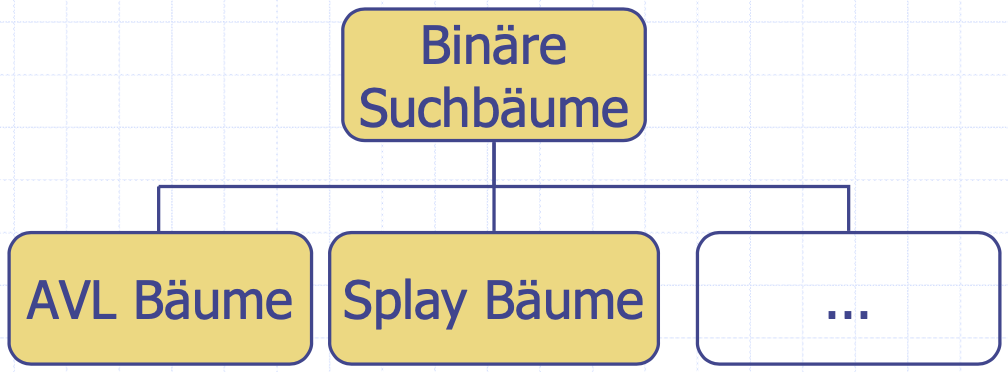
\includegraphics[scale=.15]{graphic/01 BinarySearchTrees/Ubersicht.png}
    \vspace{-4pt}
\end{center}
\begin{itemize}
    \item Binärer Baum, welcher Keys in seinen internen Knoten speichert
    \item Die Inorder-Traversierung besucht die Keys in nicht absteigender Folge
    \item Externe Knoten (Blatt-Knoten) speichern keine Daten
\end{itemize}

\subsection{Suche}
\begin{itemize}
    \item Suche nach dem Key k beginnen bei Root
    \item nächste Knoten ist, hängt vom Resultat des Vergleiches von k mit dem Key des aktuellen Knotens ab
    \item Wenn ein Blatt erreicht $\rightarrow$ Key nicht gefunden $\rightarrow$ geben v zurück
\end{itemize}
\begin{center}
    \vspace{-8pt}
    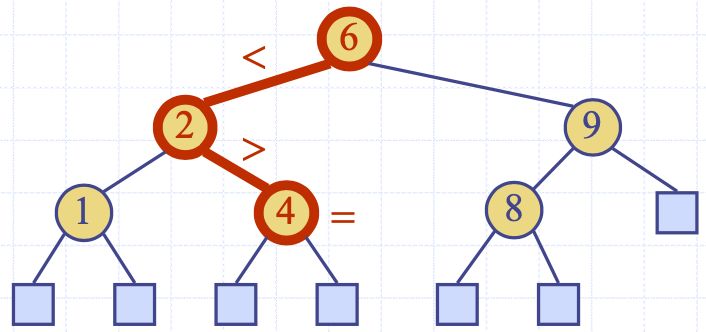
\includegraphics[scale=.3]{graphic/01 BinarySearchTrees/suche.png}
\end{center}
\begin{lstlisting}
Algorithm TreeSearch(k, v)
    if T.isExternal (v)     //Bsp: t.left(8)
        return v
    if k < key(v)           //Bsp: key(6)
        return TreeSearch(k, T.left(v))
    else if k = key(v)      //Bsp: key(4)
        return v
    else { k > key(v) }     //Bsp: key(2)
        return TreeSearch(k, T.right(v))
\end{lstlisting}

\subsection{Einfügen}
\begin{itemize}
    \item suchen wir zuerst den Key k
\end{itemize}
\subsubsection{Fall 1:}
\begin{itemize}
    \item k noch nicht im Baum und w ist Blatt, welches mit der Suche gefunden wird
    \item fügen k beim Knoten w ein und expandieren w in einen internen Knoten
\end{itemize}
Beispiel: insert(5)
\vspace{-8pt}
\begin{multicols}{2}
    \includegraphics[scale=.25]{graphic/01 BinarySearchTrees/einfügen1.1.png}
    %\columbreak
    \includegraphics[scale=.25]{graphic/01 BinarySearchTrees/einfügen1.2.png}
\end{multicols}
\vspace{-8pt}

\subsubsection{Fall 2:}
\begin{itemize}
    \item k ist schon im Baum vorhanden
    \item im linken Teilbaum von k wird weitergesucht bis auf Blattknoten w stösst
    \item fügen k beim Knoten w ein und expandieren w in einen internen Knoten
\end{itemize}
Beispiel: insert(2)
\vspace{-8pt}
\begin{multicols}{2}
    \includegraphics[scale=.25]{graphic/01 BinarySearchTrees/einfügen2.1.png}
    \includegraphics[scale=.25]{graphic/01 BinarySearchTrees/einfügen2.2.png}
\end{multicols}
\vspace{-8pt}

\subsection{Löschen}
\begin{itemize}
    \item suchen wir zuerst den Key k
    \item drei Fälle unterscheiden
\end{itemize}
\subsubsection{Fall 1 - ein Knoten mit zwei Blatt Kinder}
\begin{itemize}
    \item v ist der entsprechende Knoten
    \item v und w vom Baum gelöscht mit der Operation removeExternal(w) $\rightarrow$ Eltern-Knoten durch w'' ersetzt
\end{itemize}
Beispiel: remove(4)
\vspace{-8pt}
\begin{center}
    \includegraphics[scale=.25]{graphic/01 BinarySearchTrees/löschen1.png}
\end{center}
\vspace{-8pt}

\subsubsection{Fall 2 - ein Knoten mit einem Blatt Kind}
\begin{itemize}
    \item v ist der entsprechende Knoten
    \item v und w vom Baum gelöscht mit der Operation removeExternal(w) $\rightarrow$ Eltern-Knoten durch Knoten 5 ersetzt
\end{itemize}
Beispiel: remove(4)
\vspace{-8pt}
\begin{center}
    \includegraphics[scale=.25]{graphic/01 BinarySearchTrees/löschen2.png}
\end{center}
\vspace{-8pt}

\subsubsection{Fall 3 - ein Knoten ohne Blatt Kinder}
\begin{itemize}
    \item finde den internen Knoten w, welcher v in der Inorder Traversierung folgt
    \item kopiere key(w) in den Knoten v
    \item lösche den Knoten w und sein linkes Kind z mit removeExternal(z)
\end{itemize}
Beispiel: remove(3)
\vspace{-8pt}
\begin{multicols}{2}
    \includegraphics[scale=.25]{graphic/01 BinarySearchTrees/löschen3.1.png}
    \includegraphics[scale=.25]{graphic/01 BinarySearchTrees/löschen3.2.png}
\end{multicols}
\vspace{-8pt}

\subsection{Performance}
\begin{itemize}
    \item Speicher ist O(n)
    \item find, insert und remove benötigen O(h)
    \item Höhe h:
    \begin{itemize}
        \item Worst Case: O(n) $\rightarrow$ serieller Baum
        \item Best Case: O(log n) $\rightarrow$ schöner Baum
    \end{itemize}
\end{itemize}

\subsection{Implementierung}
\subsubsection{Baum}
\begin{center}
    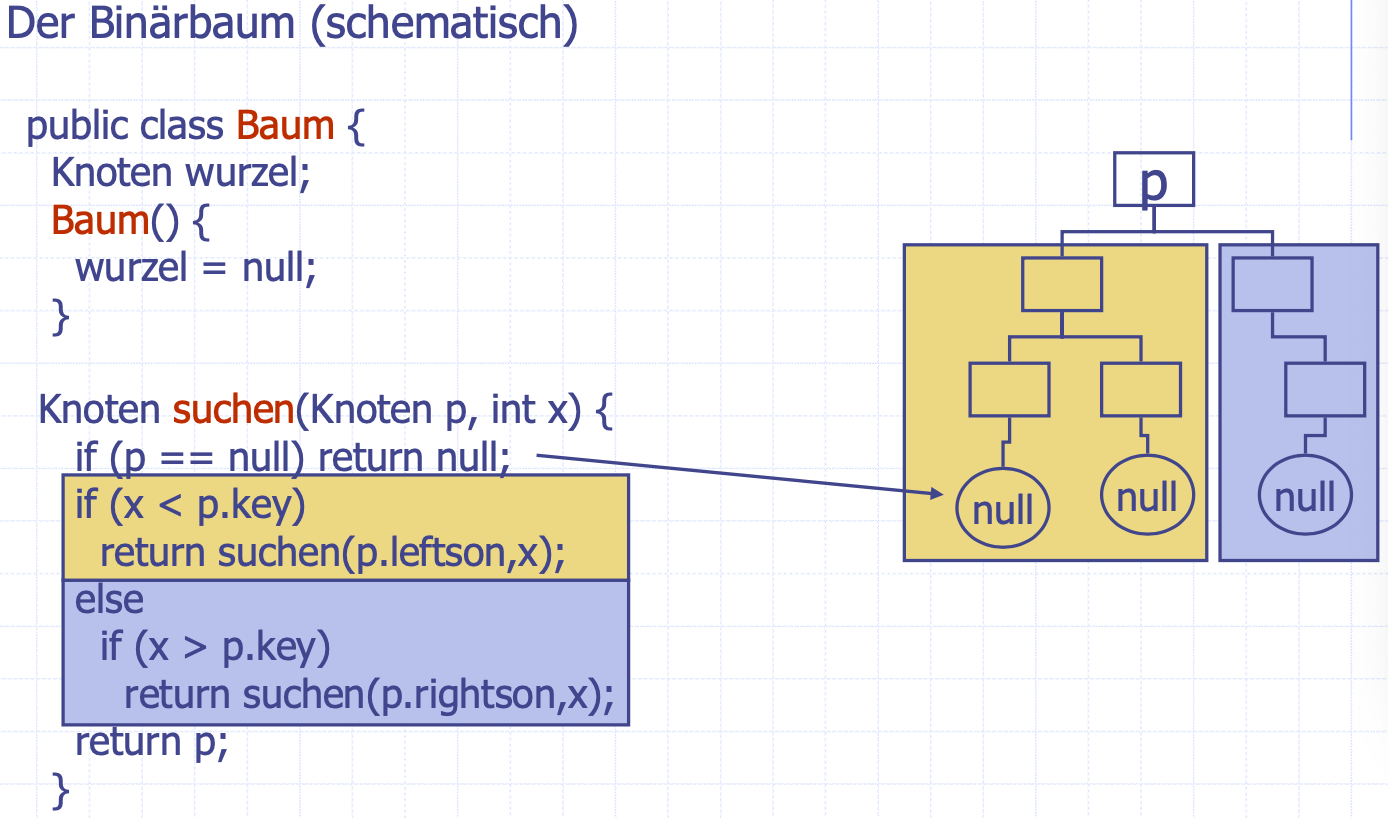
\includegraphics[scale=.22]{graphic/01 BinarySearchTrees/Baum.png}
\end{center}
\vspace{-8pt}

\subsubsection{einfügen}
\begin{center}
    \includegraphics[scale=.3]{graphic/01 BinarySearchTrees/einfügen.png}
\end{center}
\vspace{-12pt}

\subsubsection{entfernen}
\begin{center}
    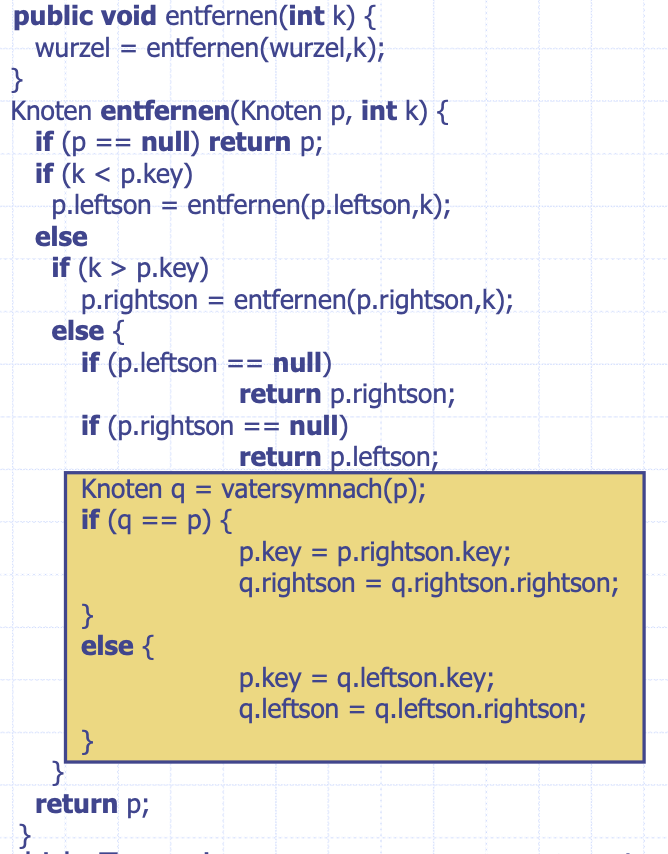
\includegraphics[scale=.3]{graphic/01 BinarySearchTrees/entfernen.png}
\end{center}
\vspace{-8pt}

\subsubsection{inorder}
\begin{center}
    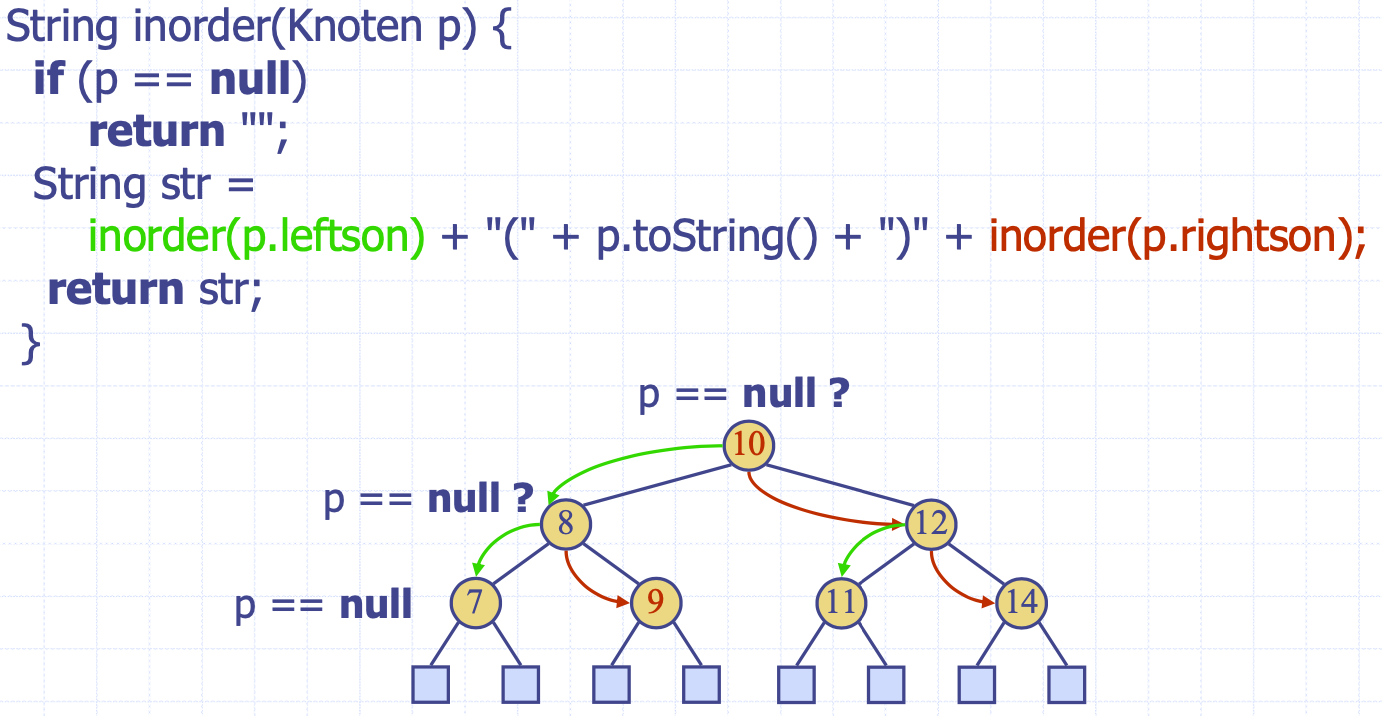
\includegraphics[scale=.22]{graphic/01 BinarySearchTrees/inorder().png}
\end{center}


\paragraph{Laufzeit}
Sortieren von Zahlen durch einfügen in binären Suchbaum und anschliessend durch INORDER-TREE-WALK sortiert ausgeben:\\

\textbf{Worst-Case (1,2,3,4,5,6, ...,n)}\\
Für Element x auch x Schritte für einfügen:\\
$\sum_{i=1}^{n} i=\frac{n(n+1)}{2}$\\
Laufzeit $O(n^2)$\\

\textbf{Best-Case (vollständiger Binärbaum entsteht)}\\
Für Element x nur $log_2$ (x) Schritte für einfügen:\\
$\sum_{i=1}^{n}\left\lfloor\log _{2}(i)\right\rfloor \leq \sum_{i=1}^{n} \log _{2}(i)$\\
Laufzeit $O(n$ $log_2 (n))$\\

\textbf{Auslesen)}\\
Das Auslesen aus dem Binärbaum erfolgt in beiden Fällen mit Inorder-Tree-Walk:\\
Laufzeit $O(n)$\\

\textbf{Total)}\\
Totale Laufzeit nicht abhängig von Auslesen, da  $O(n^2)$ und $O(n$ $log_2 (n))$ höher sind als $O(n)$. 
\newpage
    \section{AVL Trees}
\subsection{Definition}
\begin{itemize}
    \item ist ein binärer Suchbaum
    \item die Höhe der Kinder unterscheiden sich höchstens um 1
    \item AVL Bäume sind balanciert
\end{itemize}

\begin{center}
    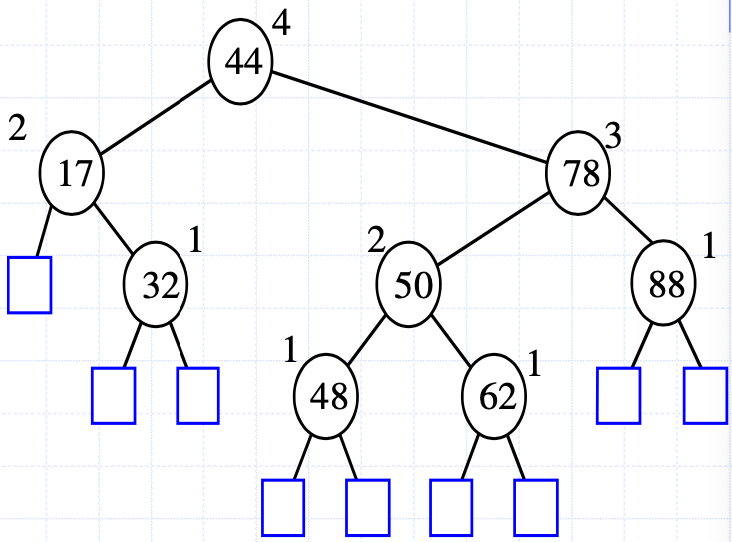
\includegraphics[scale=.25]{graphic/02 AVLTrees/definition.png}
\end{center}


\subsection{Laufzeit}
\begin{itemize}
    \item einzelne Restrukturierung O(1)
    \item find() O(log n)
    \begin{itemize}
        \item keine Restrukturierung nötig
    \end{itemize}
    \item insert() O(log n)
    \begin{itemize}
        \item find ist O(log n)
        \item eventuelle Restrukturierung baumaufwärts ist O(1)
    \end{itemize}
    \item delete ist O(log n)
    \begin{itemize}
        \item find ist O(log n)
        \item eventuelle Restrukturierungen baumaufwärts sind O(log n)
    \end{itemize}
\end{itemize}


\subsection{Höhe eines AVL Tree}
Die Höhe eines AVL Baumes T, der n Keys speichert, ist O(log(n))

\subsection{Balance}
\begin{itemize}
    \item b(k) = Höhe(links) – Höhe(rechts)
    \item b(k) ist –1, 0 oder +1
    \item Nach einfügen neuen Knotens kann gelten -2 <= b(k) <= 2
\end{itemize}


\subsection{Einfügen}
\begin{itemize}
    \item erfolgt wie beim binären Such-Baum
    \item wird immer ein externer Knoten expandiert
\end{itemize}
\subsubsection{Verletzung der Regel}
Verletzungen des AVL-Merkmals können auftreten bei:
\begin{enumerate}
    \item Einfügen eines Knotens in den linken Teilbaum des linken Sohnes
    \item Einfügen eines Knotens in den rechten Teilbaum des linken Sohnes
    \item Einfügen eines Knotens in den linken Teilbaum des rechten Sohnes
    \item Einfügen eines Knotens in den rechten Teilbaum des rechten Sohnes
\end{enumerate}
$\rightarrow$ wandern im neuen Baum aufwärts, bis den ersten Knoten x finden, dessen Grosseltern z ein unbalancierter Knoten ist.
\begin{center}
    \includegraphics[scale=.3]{graphic/02 AVLTrees/einfügen.png}
\end{center}


\subsection{Trinode Umstruktruierung}
\subsubsection{Einzel-Rotation}
\begin{center}
    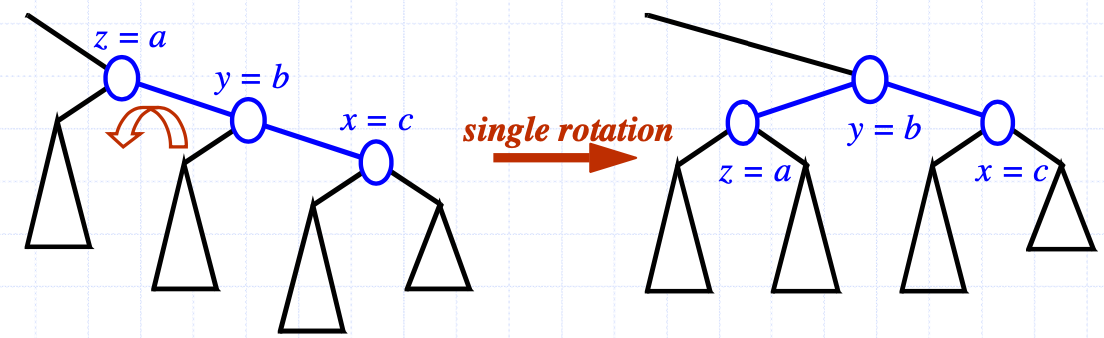
\includegraphics[scale=.22]{graphic/02 AVLTrees/Einzel-Rotationen.png}
\end{center}
\begin{lstlisting}
BinaryNode rotateWithLeftChild(BinaryNode k2) {
    BinaryNode k1 = k2.left; //Hilfsknoten
    k2.left = k1.right;
    k1.right = k2;
    return k1; }
\end{lstlisting}
\begin{lstlisting}
BinaryNode rotateWithRightChild(BinaryNode k1) {
    BinaryNode k2 = k1.right; //Hilfsknoten
    k1.right = k2.left;
    k2.left = k1;
    return k2; }
\end{lstlisting}

\subsubsection{Doppel-Rotation}
\begin{center}
    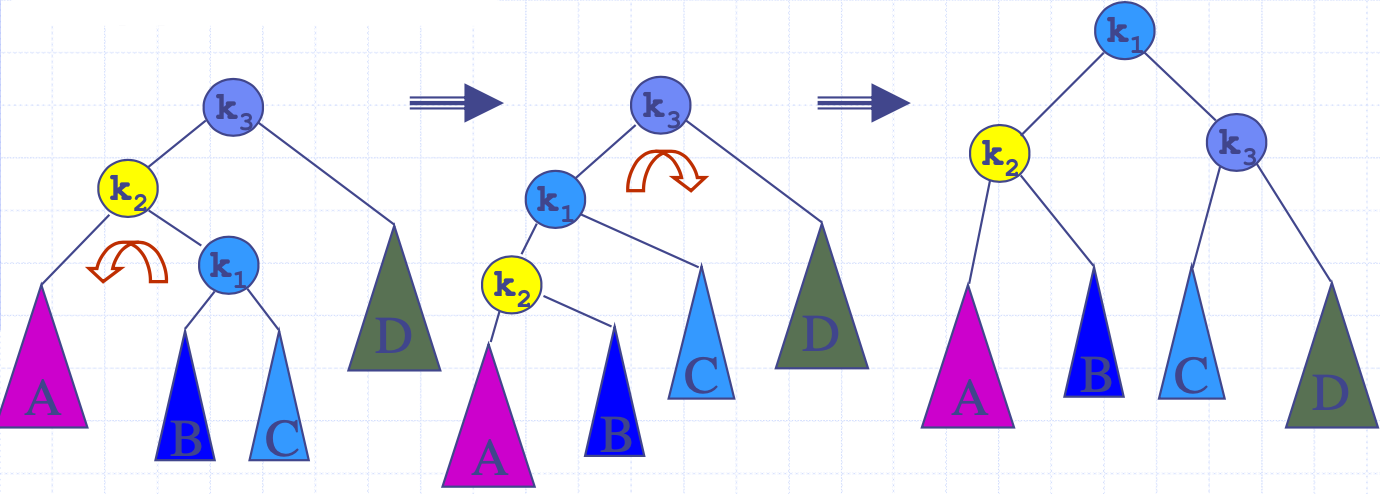
\includegraphics[scale=.22]{graphic/02 AVLTrees/Doppel-Rotationen.png}
\end{center}
\begin{lstlisting}
BinaryNode doubleRotateWithLeftChild(BinaryNode k3) {
    k3.left = rotateWithRightChild(k3.left);
    return rotateWithLeftChild(k3); }
\end{lstlisting}


\subsection{Cut/Link Restrukturierungs Algorithmus}
\subsubsection{Übersicht}
\begin{itemize}
    \item bewirkt das selbe, wie die vier obigen Rotationen
    \item Vorteil:
    \begin{itemize}
        \item keine Fallunterscheidung
        \item eleganter
    \end{itemize}
    \item Nachteil:
    \begin{itemize}
        \item komplexerer Programmcode
    \end{itemize}
    \item beide Algorithmen haben die selbe Zeitkomplexität
\end{itemize}

Funktion restructure(x):
\begin{itemize}
    \item \textbf{Input:} Knoten x eines binären Suchbaumes T, welcher einen Eltern-Knoten y und einen Grosseltern-Knoten z besitzt.
    \item \textbf{Output:} restrukturierter Baum T, mit rotierten Knoten (Single oder Double) x, y und z
\end{itemize}

\subsubsection{Ablauf}
\begin{enumerate}
    \item In 7 Teile aufteilen (In-Order Traversierung)
    \item nenne Knoten um (a, b, c: gemäss In-Order)
\end{enumerate}
\vspace{-8pt}
\begin{center}
    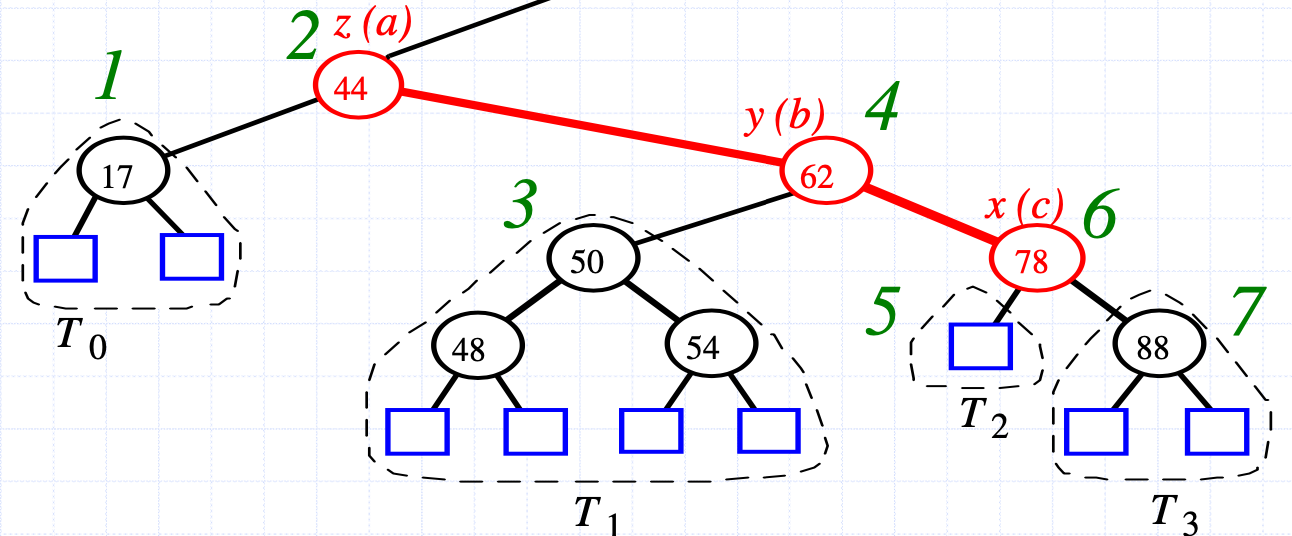
\includegraphics[scale=.28]{graphic/02 AVLTrees/Cut-Link1.png}
\end{center}
\vspace{-8pt}

\begin{enumerate}
    \setcounter{enumi}{3}
    \item kreieren ein Array mit 7 Elementen: 1 bis 7
\end{enumerate}
\vspace{-8pt}
\begin{center}
    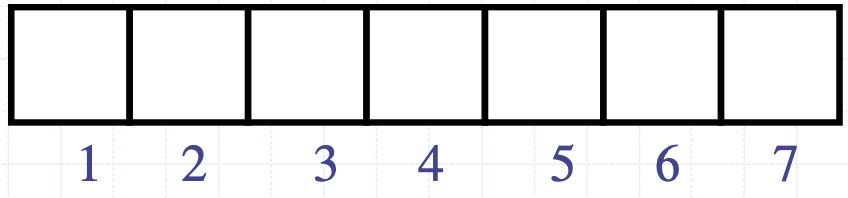
\includegraphics[scale=.2]{graphic/02 AVLTrees/Cut-Link2.png}
\end{center}
\vspace{-8pt}

\begin{enumerate}
    \setcounter{enumi}{4}
    \item schneiden 4 Bäume ab und platzieren sie in Array (In-Order)
\end{enumerate}
\vspace{-8pt}
\begin{center}
    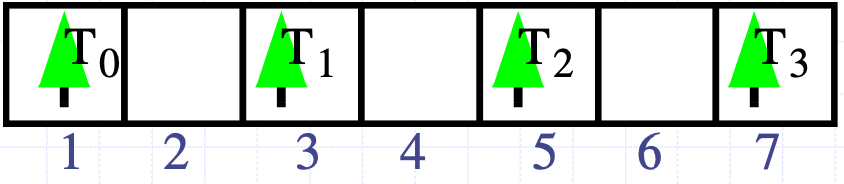
\includegraphics[scale=.2]{graphic/02 AVLTrees/Cut-Link3.png}
\end{center}
\vspace{-8pt}

\begin{enumerate}
    \setcounter{enumi}{5}
    \item stellen x,y und z (child,parent, grandparent) in In-Order in das Array
\end{enumerate}
\vspace{-8pt}
\begin{center}
    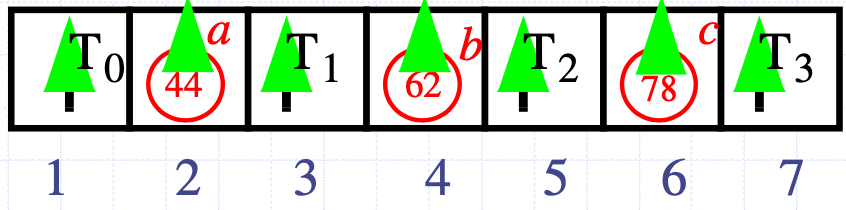
\includegraphics[scale=.2]{graphic/02 AVLTrees/Cut-Link4.png}
\end{center}
\vspace{-8pt}

\begin{enumerate}
    \setcounter{enumi}{6}
    \item bauen Baum schrittweise wieder auf
\end{enumerate}
\vspace{-8pt}
\begin{center}
    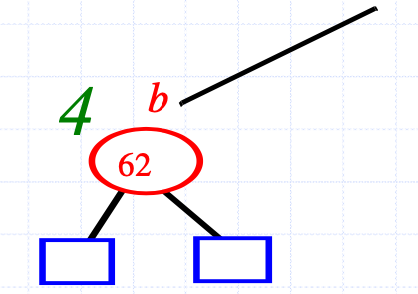
\includegraphics[scale=.25]{graphic/02 AVLTrees/Cut-Link5.png}
\end{center}
\vspace{-8pt}

\begin{enumerate}
    \setcounter{enumi}{7}
    \item setzen Element 2 (a) und Element 6 (c) als Kinder von 4 im Baum ein
\end{enumerate}
\vspace{-8pt}
\begin{center}
    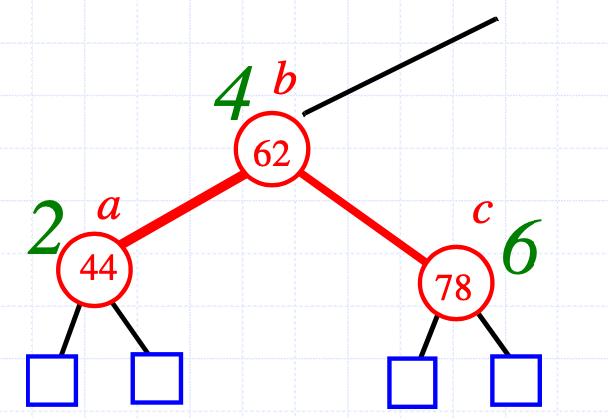
\includegraphics[scale=.2]{graphic/02 AVLTrees/Cut-Link6.png}
\end{center}
\vspace{-8pt}

\begin{enumerate}
    \setcounter{enumi}{8}
    \item Schluss setzen wir 1,3,5 und 7 als Kinder von 2 und 6 in den Baum ein
\end{enumerate}
\vspace{-8pt}
\begin{center}
    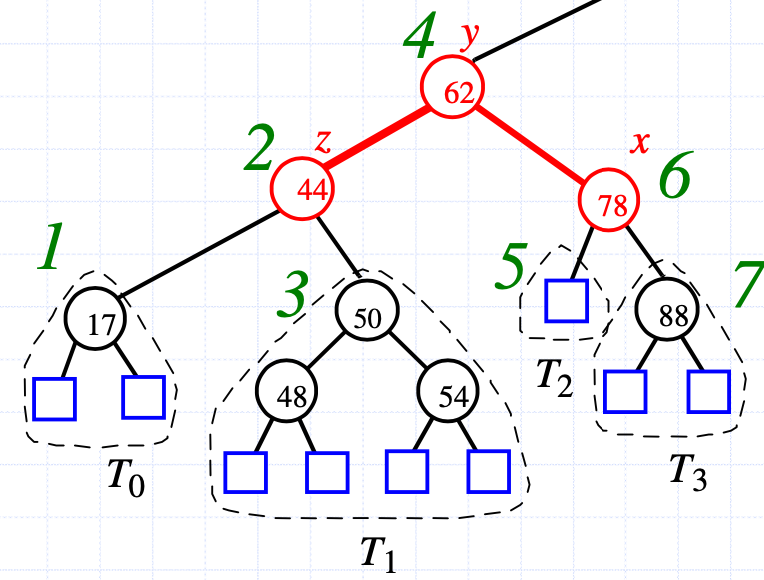
\includegraphics[scale=.2]{graphic/02 AVLTrees/Cut-Link7.png}
\end{center}
\vspace{-8pt}


\subsection{Löschen}
\begin{itemize}
    \item beginnt wie im binären Suchbaum
    \item Eltern-Knoten kann jetzt Balance aus dem Gleichgewicht bringen
\end{itemize}
\subsubsection{Balancierung nach löschen}
\begin{itemize}
    \item z = erste unbalancierte Knoten
    \item y = Kind von z mit der grösseren Höhe
    \item x = das Kind von y mit der grösseren Höhe
    \item Aufruf von restructure(x) um die Balance von z herzustellen
    \item Umstrukturierung kann eine neue Unbalance hervorrufen
    \item Balance weiter geprüft werden bis die Wurzel von T erreicht ist
\end{itemize}
\begin{center}
    \includegraphics[scale=.2]{graphic/02 AVLTrees/Balancierung nach dem Löschen.png}
\end{center}
\begin{lstlisting}
private boolean isBalanced(Position p) {
    int bf=height(T.leftChild(p))- height(T.rightChild(p));
    return ((-1 <= bf) && (bf <= 1));}
\end{lstlisting}


\newpage
    \section{Splay Trees}
\subsection{Definition}
\begin{itemize}
    \item binärer Suchbaum
    \item nach Zugriff auf Knoten $\rightarrow$ dieser zur Root
    \item Inorder-Traversierung retourniert die Keys in geordneter Folge
\end{itemize}

\subsection{Laufzeit}
Splaying-Cost: O(h)
\begin{itemize}
    \item Durschnittlich: O(log n)
    \item Worst Case: O(n)
\end{itemize}

\subsection{Splaying}
\begin{itemize}
    \item neue operation: splay
    \item Rotationen nach jeder Operation (sogar bei der Suche)
    \item Bewegen eines Knoten zur Root unter Benutzung von Rotationen
\end{itemize}

\begin{itemize}
    \item x ist das linke Kind von seinem Eltern-Knoten, welcher selber ein rechtes Kind ist von seinem Eltern-Knoten
    \item y ist x’s Eltern-Knoten
    \item z ist y’s Eltern-Knoten
\end{itemize}

\vspace{-8pt}
\begin{center}
    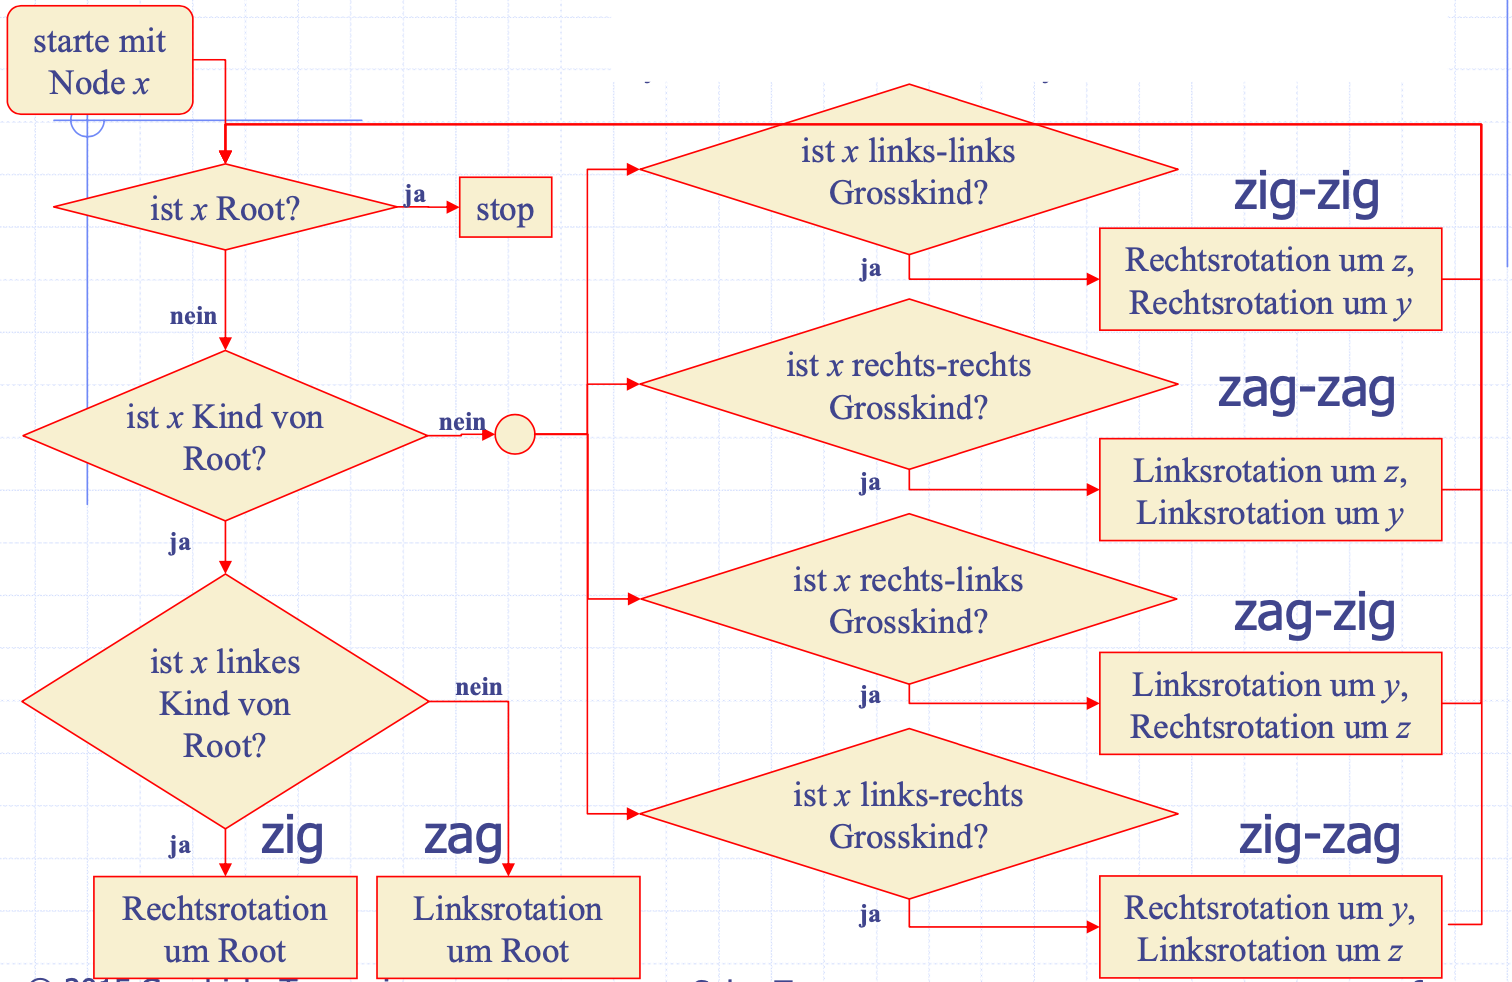
\includegraphics[scale=.2]{graphic/03 SplayTrees/splay.png}
    \includegraphics[scale=.2]{graphic/03 SplayTrees/splay fälle.png}
\end{center}
\vspace{-8pt}

\subsection{Suchen}
Suche geht den Baum abwärts bis zu einem gesuchten Entry oder einem externer Knoten

\subsection{Löschen}
\begin{center}
    \includegraphics[scale=.2]{graphic/03 SplayTrees/löschen}
\end{center}
\vspace{-8pt}

\subsection{Wer wird gesplayed?}
\begin{center}
    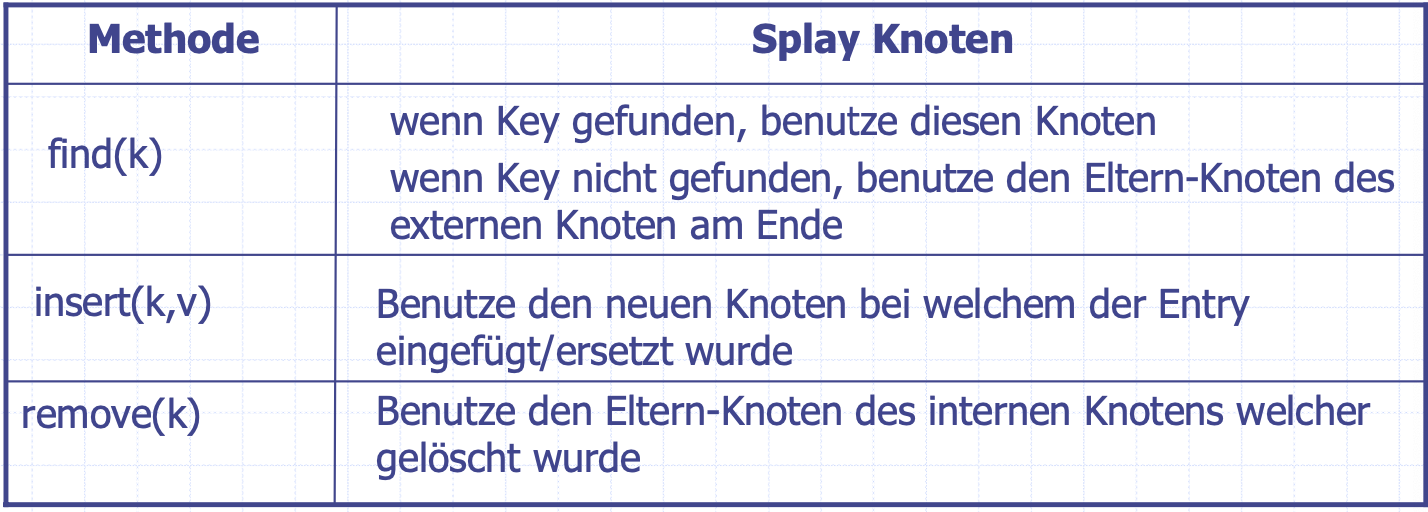
\includegraphics[scale=.25]{graphic/03 SplayTrees/who.png}
\end{center}


    \section{Merge Sort}

\subsection{Definition}
\begin{itemize}
    \item Sortieralgorithmus basierend auf Divide-and-Conquer
    \item Wie bei Heap-Sort:
    \begin{itemize}
        \item Benutzung eines Comparators
    \end{itemize}
    \item Anders als beim Heap-Sort:
    \begin{itemize}
        \item keine Benutzung einer Priority-Queue
        \item Zugriff auf Daten sequentiell (geeignet zum Sortieren von Daten auf der Disk)
    \end{itemize}
\end{itemize}

\subsubsection{Divide-and-Conquer (Teile- und-Herrsche)}
Ein generelles Paradigma beim Design von Algorithmen:
\begin{itemize}
    \item \textbf{Divide:} Input-Daten S in zwei getrennte Teilmengen S1 und S2 aufteilen
    \item \textbf{Recur (Wiederhole):} die Teilprobleme mit S1 and S2 rekursiv lösen
    \item \textbf{Conquer:} mischen der Lösungen von S1 und S2 in die Lösung von S
\end{itemize}

\subsection{Laufzeit}
\begin{itemize}
    \item Die Höhe h des Merge-Sort Baumes ist O(log n)
    \item Der Gesamt-Aufwand aller Knoten einer Tiefe i ist O(n)
    \item totale Laufzeit des Merge-Sort ist O(n * log(n))
\end{itemize}


\subsection{Algorithmus}
\begin{itemize}
    \item Input-Sequenz S
    \item n Elementen
    \item 3 Schritte:
    \begin{itemize}
        \item \textbf{Divide:} S in zwei Sequenzen S1 und S2 von je n/2 Elemente aufteilen
        \item \textbf{Recur:} rekursiv S1 und S2 sortieren
        \item \textbf{Conquer:} S1 und S2 in eine sortierte Sequenz mischen
    \end{itemize}
\end{itemize}
\begin{lstlisting}
Algorithm mergeSort(S, C)
    Input sequence S with n elements, comparator C
    Output sequence S sorted according to C
    if S.size() > 1
        (S1, S2) <- partition(S, n/2)
        S1 <- mergeSort(S1, C)
        S2 <- mergeSort(S2, C)
        S <- merge(S1, S2)
    return S
\end{lstlisting}
Mischen von zwei sortierten Sequenzen A und B in die sortierte Sequenz S, enthaltend die Vereinigung der Elemente von A und B\\
Mischen zweier sortierter Sequenzen von je n/2 Elemente mit double-linked Listen: O(n) Laufzeit \\
\subsection{Mischen zweier sortierter Sequenzen}

\begin{lstlisting}
Algorithm merge(A, B)
    Input sequences A and B with n/2 elements each
    Output sorted sequence of A £$\bigcup$£  B

    S <- empty sequence
    while !A.isEmpty() && !B.isEmpty()
        if A.first().element() < B.first().element()
            S.insertLast(A.remove(A.first()))
        else
            S.insertLast(B.remove(B.first()))
    while !A.isEmpty()
        S.insertLast(A.remove(A.first()))
    while !B.isEmpty()
        S.insertLast(B.remove(B.first()))
    return S
\end{lstlisting}

\subsection{Merge-Sort Baum}
\begin{itemize}
    \item Die Ausführung eines Merge-Sort kann als binärer Baum dargestellt werden
    \item Jeder Knoten representiert einen rekursiven Aufruf des Merge- Sort und enthält:
    \begin{itemize}
        \item unsortierte Sequenz vor der Ausführung und der Aufteilung
        \item sortierte Sequenz nach dem Ende der Ausführung
    \end{itemize}
    \item Wurzel entspricht dem initialen Aufruf
    \item Blätter sind Aufrufe auf Teilsequenzen der Grösse 0 oder 1
\end{itemize}
\begin{center}
    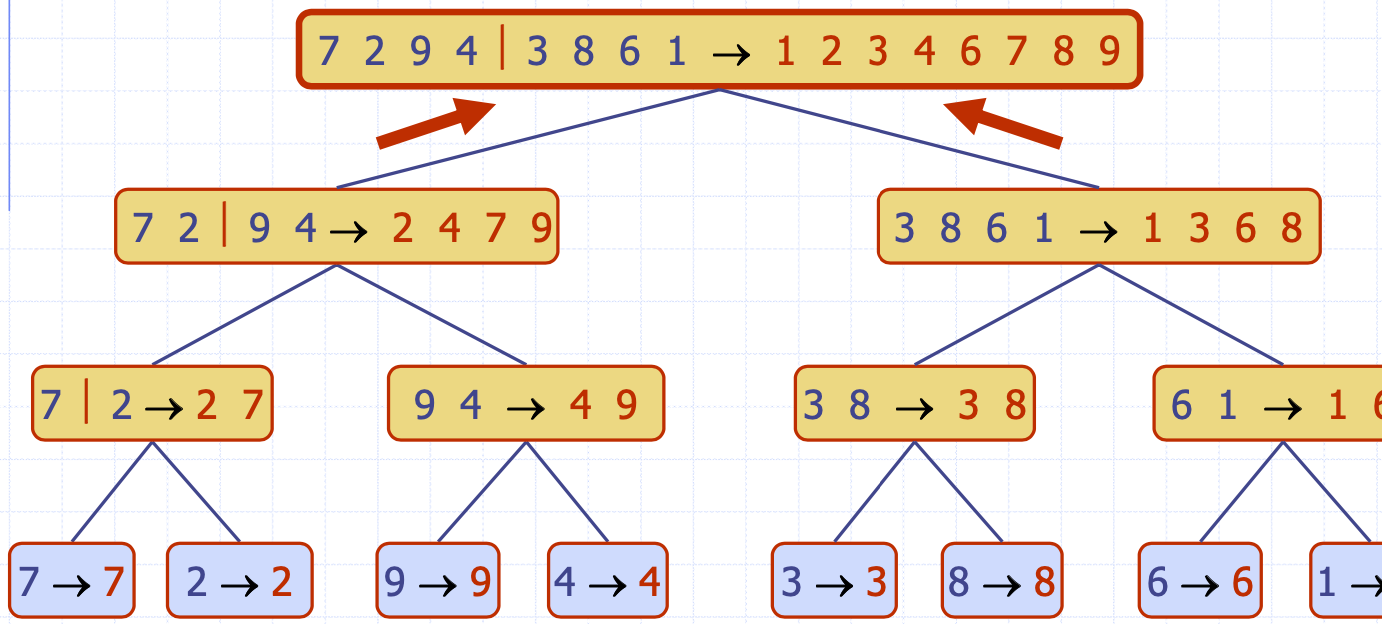
\includegraphics[scale=.2]{graphic/04 MergeSort/merge sort.png}
\end{center}

\newpage
    \section{Quick Sort}


\subsection{Definition}
\begin{itemize}
    \item basierend auf dem Divide-and-Conquer
    \item \textbf{Devide:} Auswahl eines zufälligen Elementes x (Pivot) und Aufteilung von S in:
    \begin{itemize}
        \item L Elemente kleiner als x
        \item E Elemente gleich x
        \item G Elemente grösser als x
    \end{itemize}
    \item \textbf{Recur:} sortiere L und G
    \item \textbf{Conquer:} vereine L, E and G
\end{itemize}
\vspace{-8pt}
\begin{center}
    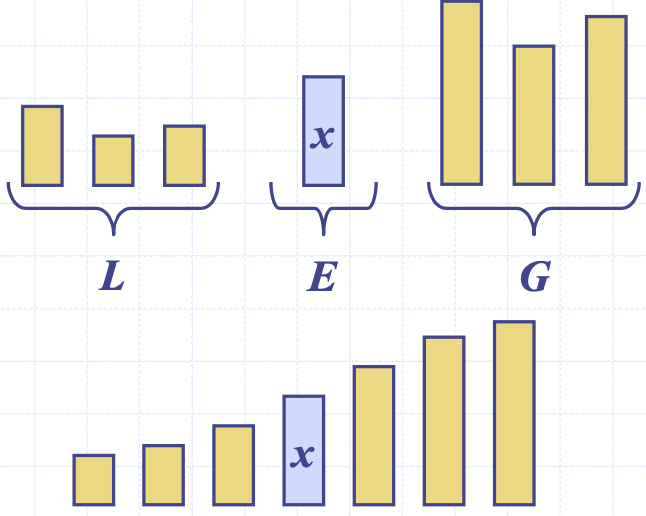
\includegraphics[scale=.3]{graphic/05 QuickSort/def.png}
\end{center}
\vspace{-8pt}


\subsection{Laufzeit}
\begin{itemize}
    \item Worst Case: $O(n^2)$ $\rightarrow$ Pivot Min- oder Max-Element
    \item Erwartet: O(n log (n))
    \begin{itemize}
        \item Good call: Länge von L und G sind beide kleiner als 3s/4
        \item Bad call: entweder L oder G ist länger als 3s/4 (s = länge)
        \item Aufruf ist ‘good’ mit einer Wahrscheinlichkeit von 1/2
    \end{itemize}
\end{itemize}
\begin{center}
    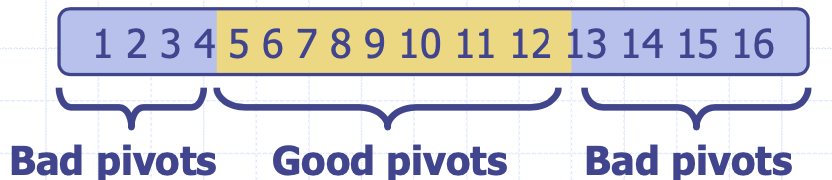
\includegraphics[scale=.3]{graphic/05 QuickSort/laufzeit.png}
\end{center}
\vspace{-8pt}


\subsection{Partitionierung}
\begin{itemize}
    \item Aufteilung der Input- Sequence:
    \begin{itemize}
        \item Entfernen von jeweils einem Element y von S
        \item einfügen von y in L, E oder G, abhängig vom Resultat des Vergleiches mit dem Pivot x
    \end{itemize}
    \item Aufteilung des Quick-Sort benötigt somit: O(n)
\end{itemize}


\subsection{Quick Sort Tree}
Ausführung eines Quick-Sort kann als binärer Baum dargestellt werden
\begin{itemize}
    \item Jeder Knoten repräsentiert einen rekursiven Aufruf des Quick- Sort und enthält:
    \begin{itemize}
        \item unsortierte Sequenz vor der Ausführung und sein Pivot
        \item sortierte Sequenz und sein Pivot nach dem Ende der Ausführung
    \end{itemize}
    \item Wurzel entspricht dem initialen Aufruf
    \item Blätter sind Aufrufe auf Teilsequenzen der Grösse 0 or 1
\end{itemize}
\vspace{-8pt}
\begin{center}
    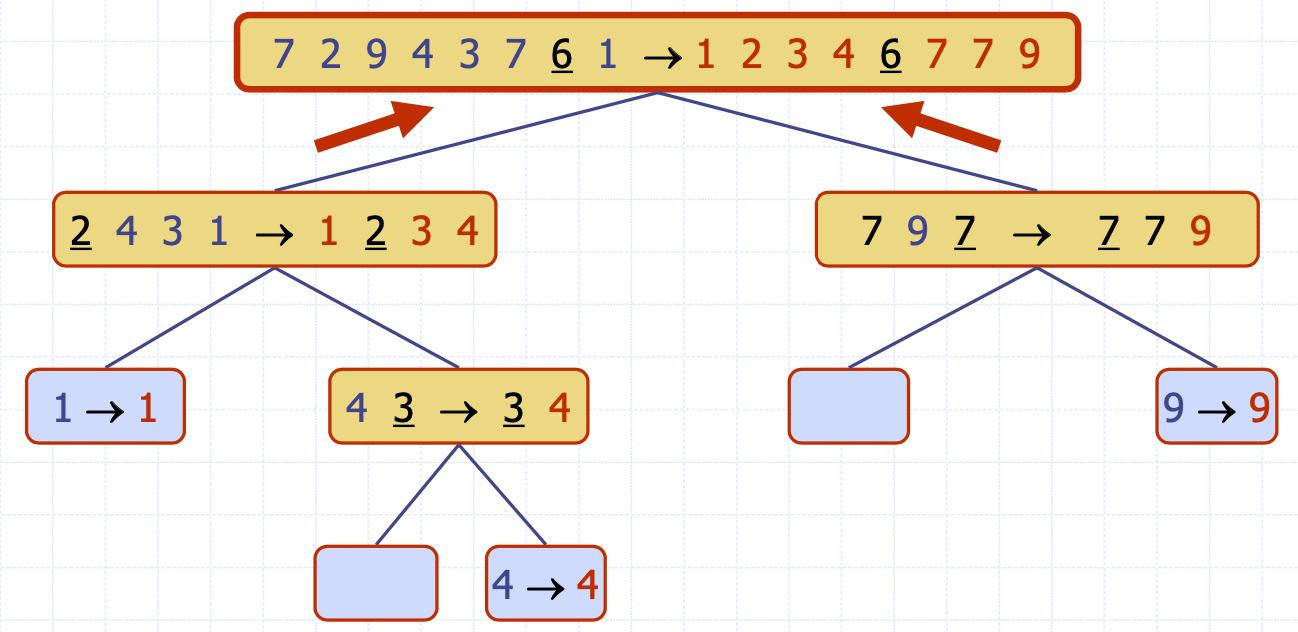
\includegraphics[scale=.2]{graphic/05 QuickSort/Quick Sort Tree.png}
\end{center}
\vspace{-8pt}


\subsection{In-Place Quick-Sort}
\begin{itemize}
    \item Quick-Sort kann ‘In-Place’ implementiert werden
    \item Partitionierungs-Schritt werden die Elemente der Input- Sequenz derart umgeordnet, dass:
    \begin{itemize}
        \item Elemente kleiner als das Pivot einen Index kleiner als h haben
        \item Elemente gleich dem Pivot einen Index zwischen h und k haben
        \item Elemente grösser als das Pivot einen Index grösser als k haben
    \end{itemize}
    \item rekursiven Calls betrachten
    \begin{itemize}
        \item Elemente mit Index kleiner als h
        \item Elemente mit Index grösser als k
    \end{itemize}
\end{itemize}
\subsubsection{Implementierung}
\begin{itemize}
    \item Partitionierung mit Benutzung zweier Indices um S in L und E \& G aufzuteilen.
\end{itemize}
\begin{center}
    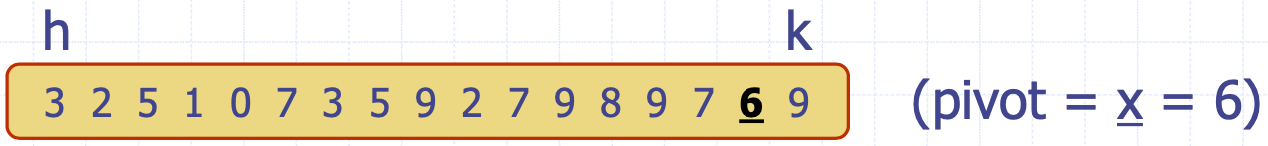
\includegraphics[scale=.2]{graphic/05 QuickSort/In-Place1.png}
\end{center}
\begin{itemize}
    \item Wiederholung bis h und k sich kreuzen:
    \begin{itemize}
        \item h nach rechts bis zu einem Element >= x
        \item k nach links bis zu einem Element < x
        \item Wenn h und k noch nicht gekreuzt: Elemente mit Indizes h und k vertauschen
    \end{itemize}
\end{itemize}
\vspace{-8pt}
\begin{center}
    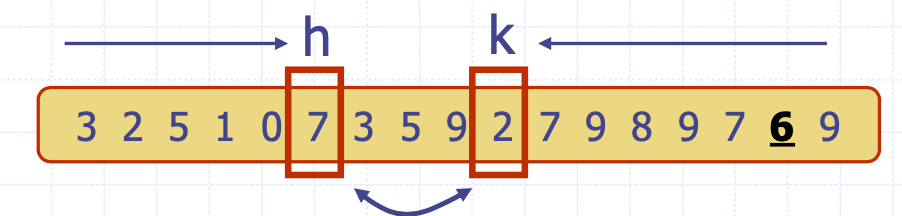
\includegraphics[scale=.2]{graphic/05 QuickSort/In-Place2.png}
\end{center}
\vspace{-8pt}
\begin{itemize}
    \item Pivot mit Element an Index h vertauschen
\end{itemize}


\section{Zusammenfassung Sortier-Algorithmen}
\begin{center}
    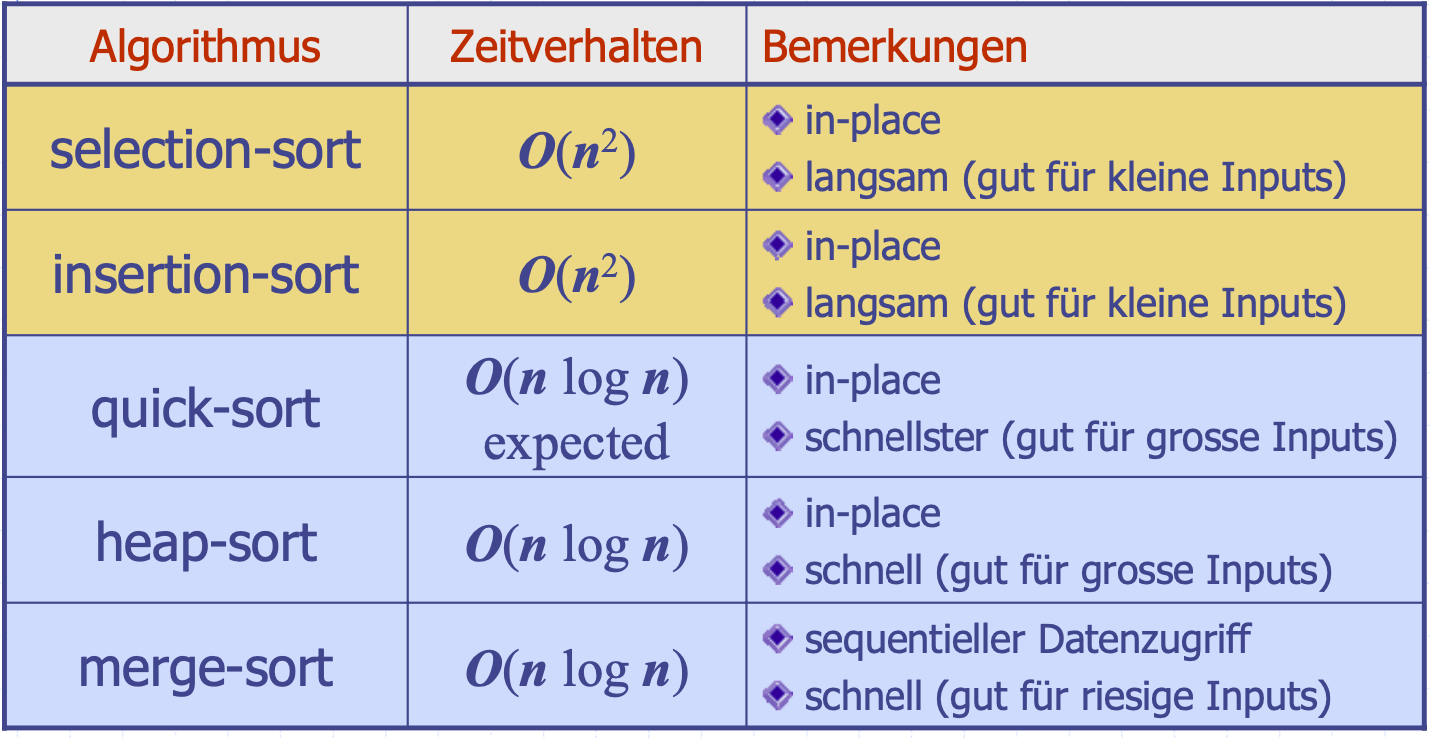
\includegraphics[scale=.25]{graphic/05 QuickSort/zfsg.png}
\end{center}
\vspace{-8pt}


    \section{Sorting Lower Bound}

\subsection{Definition}
\begin{itemize}
    \item Viele Sortier-Algoritmen sind vergleichsbasiert
    \item soll eine untere Grenze (Lower Bound) der Laufzeit hergeleitet werden für alle Algorithmen, welche Vergleiche benutzen um n Elemente $x_1, x_2, ..., x_n$ zu sortieren.
\end{itemize}

\subsection{Laufzeit}
\begin{itemize}
    \item Jeder Vergleichs-basierte Sortier-Algorithmus hat eine minimale Laufzeit von: log (n!)
    \item Jeder solch Algorithmus hat somit eine Laufzeit von
    mindestens (gem. Starling-Annäherung): O(n log(n))
\end{itemize}

\subsection{Zählen der Vergleiche}
\begin{itemize}
    \item zählen die Anzahl der Vergleiche
    \item Jeder mögliche Durchgang des Algorithmus korrespondiert mit einem Wurzel-zu-Blatt Pfad ein einem Entscheidungs-Baum
\end{itemize}


\subsection{Höhe des Entscheidungs-Baumes}
\begin{itemize}
    \item Höhe des Entscheidungs-Baumes entspricht der unteren Grenze der Laufzeit
    \item Jede mögliche Input-Permutation führt zu einem anderen Pfad
    \begin{itemize}
        \item wenn dies nicht so wäre, hätte ein Input ...4...5... die selbe Ausgangs-Ordnung wie ...5...4...(was falsch wäre)
    \end{itemize}
    \item Da n!=1*2*...*n Blätter vorhanden sind, beträgt die Höhe mindestens log(n!)
\end{itemize}
\vspace{-8pt}
\begin{center}
    \includegraphics[scale=.2]{graphic/06 SortingLowerBound/höhe.png}
\end{center}
\vspace{-8pt}

\vfill
$ $
\columnbreak

    \section{Bucket Sort}
\subsection{Definition}
\begin{itemize}
    \item S. Sequenz (Key, Element) Entries mit Keys im Bereich [0, N-1]
    \item n: Anzahl Entries
    \item benutzt die Keys als Index in einen Hilfs-Array B von Sequenzen
    \begin{itemize}
        \item \textbf{Phase 1} Sequenz S leeren durch Verschieben jedes Entry (k, o) in sein Bucket B[k]
        \item \textbf{Phase 2} Für i = 0, ..., N - 1 verschiebe die Entries des Buckets B[i] an das Ende der Sequenz S
    \end{itemize}
\end{itemize}
\vspace{-8pt}
\begin{center}
    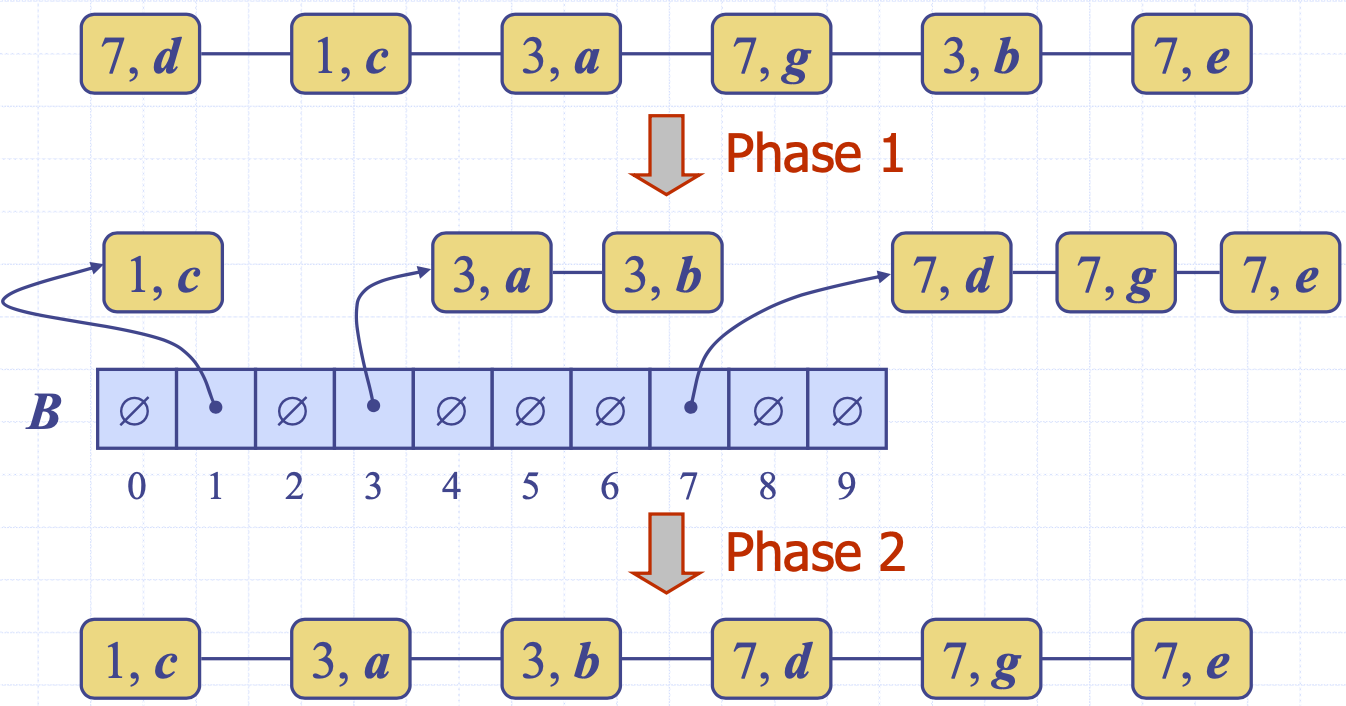
\includegraphics[scale=.22]{graphic/07 RadixSort/bucket.png}
\end{center}
\vspace{-8pt}

\subsection{Laufzeit}
\begin{itemize}
    \item Phase 1 benötigt O(n) Zeit
    \item Phase 2 benötigt O(n + N) Zeit
    \item Bucket-Sort benötigt O(n + N) Zeit
\end{itemize}

\subsection{Eigenschaften}
\subsubsection{Key}
\begin{itemize}
    \item Keys werden als Indices in einem Array benutzt und können somit nicht beliebige Objekte sein
    \item kein externer Comparator nötig
\end{itemize}
\subsubsection{Stabilität}
\begin{itemize}
    \item Die relative Ordnung von zwei Entries mit dem selben Key werden durch den Algorithmus nicht verändert
\end{itemize}

\subsubsection{Erweiterungen}
\begin{itemize}
    \item Integer Keys im Bereich [a, b]
    \item String-Keys aus einem Set D von möglichen Strings, wobei D eine konstante Grösse hat (z.B. die Namen der 50 U.S. Staaten)
\end{itemize}


\vfill
$ $
\columnbreak


\section{Lexikographische Sortierung}
\subsection{Definition}
\begin{itemize}
    \item d-Tupel ist eine Sequenz von d Keys (k1, k2, ..., kd), wobei Key ki als die i-te Dimension des Tupels bezeichnet wird
    \item Bsp: Die kartesischen Koordinaten eines Punktes im Raum sind ein 3-Tupel
    \item Die lexikographische Ordnung von zwei d-Tupels ist rekursiv definiert als:
    \begin{itemize}
        \item (x1, x2, ..., xd) < (y1, y2, ..., yd)
        \item <=>
        \item $ x1<y1 \vee  x1=y1 \wedge  (x2,...,xd) < (y2,...,yd) $
    \end{itemize}
\end{itemize}

\subsection{Laufzeit}
\begin{itemize}
    \item läuft in O(d( n + N)) Zeit
\end{itemize}

\subsection{Algorithmus}
\begin{itemize}
    \item $C_i$ der Comparator welcher zwei Tupel nach ihrer i-ten Dimension vergleicht.
    \item stableSort(S, C) sei ein stabiler Sortier-Algorithmus welcher den Comparator C benutzt
    \item Lexikographische-Sortierung sortiert eine Sequenz von d- Tupeln in lexikographischer Ordnung, indem d-mal stableSort, je einmal pro Dimension, durchgeführt wird
    \item Lexikographische-Sortierung läuft in O(d*T(n)) Zeit, wobei T(n) die Laufzeit von stableSort ist
\end{itemize}


\paragraph{Anwendung}
\begin{enumerate}
    \item Anzahl Buchstaben pro Klammer Zählen (hier 3)
    \item beginnend bei i = 3 [jeweils letzter Buchstabe]
    \item sortierung der Klammern nach Klammer[i]
    \item i - 1
    \item wiederholen bis i = 1
\end{enumerate}
\begin{center}
    Beispiel 1:\\
    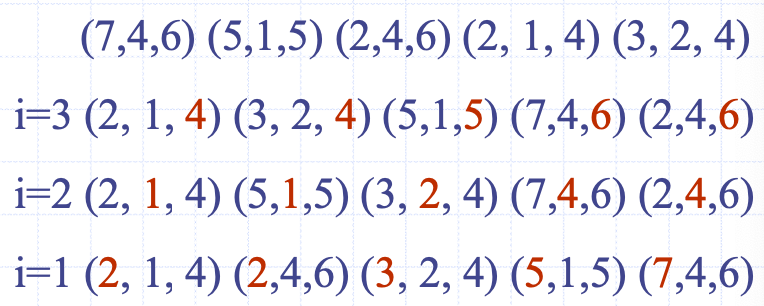
\includegraphics[scale=.3]{graphic/07 RadixSort/lexi.png}\\
    \vspace{6pt}
    Beispiel 2:\\
    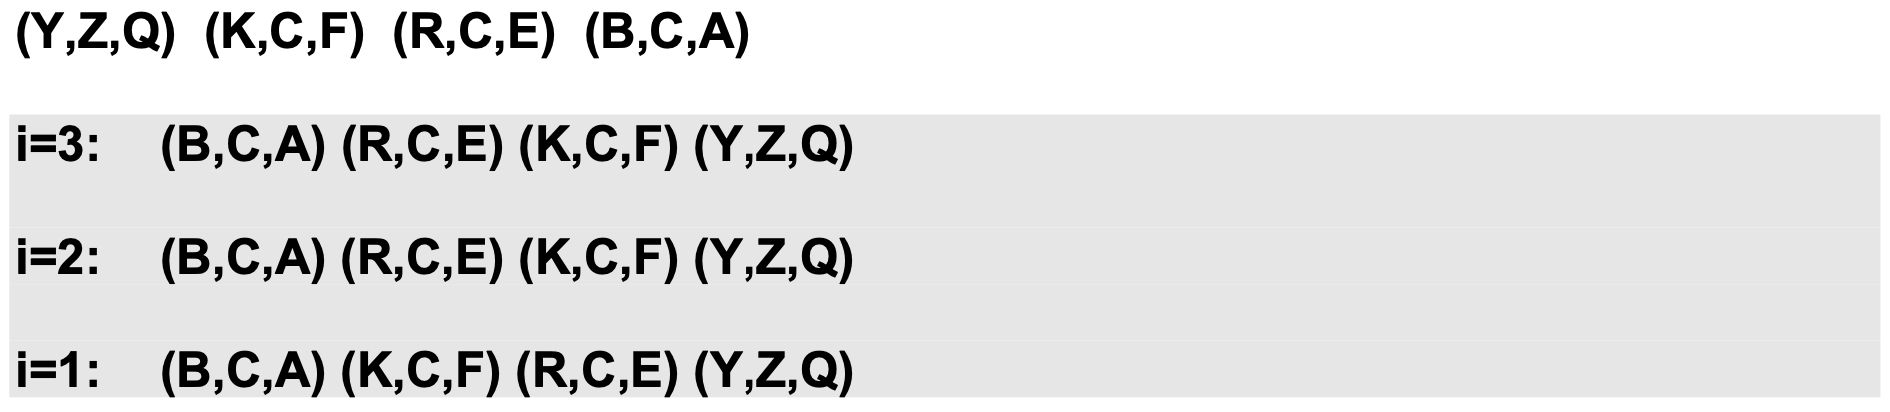
\includegraphics[scale=.19]{graphic/07 RadixSort/probepruefung_lexi.png}
\end{center}


\vfill
$ $
\columnbreak


\section{Radix Sort}
\subsection{Definition}
\begin{itemize}
    \item eine Spezialisierung des lexikographischen-Sort, welcher Bucket-Sort als stabilen Sortier- Algorithmus für jede Dimension benutzt
    \item ist anwendbar für Tupel mit Integer-Keys im Bereich [0, N - 1] in jeder Dimension i
\end{itemize}

\subsection{Laufzeit}
\begin{itemize}
    \item Beispiel: eine Sequenz von 32-Bit Integers kann in linearer Zeit sortiert werden
\end{itemize}

\subsection{für Binäre Zahlen}
\begin{itemize}
    \item Gebeben sei eine Sequenz von n b-Bit Integers:\\
    $x = x_{b - 1} ... x_1x_0$
    \item Jedes Element wird als b-Tupel von Integern im Bereich {0, 1} dargestellt. Darauf wendet man den Radix-Sort mit N = 2 an
    \item Diese Anwendung des Radix-Sort-Algorithmus läuft in O(b*n) Zeit
\end{itemize}


\vspace{-8pt}
\begin{center}
    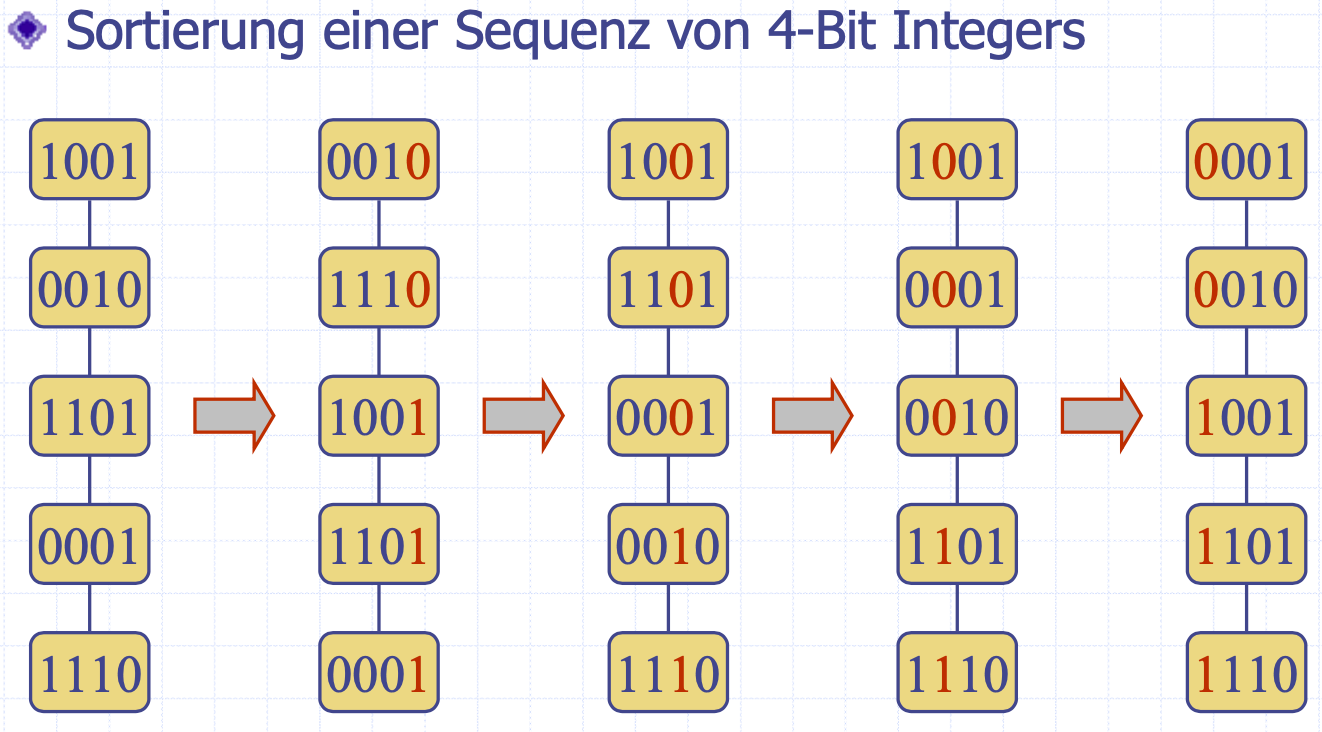
\includegraphics[scale=.2]{graphic/07 RadixSort/radix.png}
\end{center}
\vspace{-8pt}

%TODO alles nochmals schnell durchschauen, ob alles am richtigen Ort kopiert ist



\newpage
    \section{Pattern Matching}

\subsection{Brute-Force Algorithmus}
\subsubsection{Definition}
\begin{itemize}
    \item vergleicht das Pattern P mit dem Text T für jede mögliche Position von P relativ zu T, bis entweder
    \begin{itemize}
        \item eine Übereinstimmung gefunden
        \item alle möglichen Platzierungen des Patterns ausprobiert
    \end{itemize}
\end{itemize}
\subsubsection{Laufzeit}
\begin{itemize}
    \item benötigt O(nm) Zeit
    \item Worst Case:
    \begin{itemize}
        \item T = aaa...ah (Text)
        \item P = aaah (Pattern)
        \item Treten  in  Bild-Analysen  und  DNA  Sequenzenauf, Text eher nicht
    \end{itemize}
\end{itemize}
\subsubsection{Algorithmus}
\begin{lstlisting}
Algorithm BruteForceMatch(T, P)
    Input Text T der Laenge n und Pattern P der Laenge m
    Output Startindex eines Substrings von T, welcher mit P uebereinstimmt, oder -1 falls keiner gefunden wurde

    for i <- 0 to n-m { testen der i-ten Verschiebung des Patterns }
        k <- 0
        while j < m && T [i + j] = P[j]
            j <- j+1 if j = m
        return i {match bei i}
    return -1 {kein match}
\end{lstlisting}


\subsection{Boyer-Moore Algorithmus}
\subsubsection{Definition}
Basiert auf zwei Heuristiken:
    \begin{itemize}
        \item \textbf{Looking-Glass:} vergleiche P mit einer Subsequenz von T. Starte dabei am Ende des Patterns
        \item \textbf{Character-Jump:} falls bei T[i] = c keine Übereinstimmung
        \begin{itemize}
            \item falls P das Zeichen c enthält, verschiebe P bis das letzte Auftreten von c in P mit T[i] übereinstimmt.
            \item sonst, verschiebe P bis P[0] mit T[i + 1] übereinstimmt
        \end{itemize}
    \end{itemize}
\vspace{-8pt}
\begin{center}
    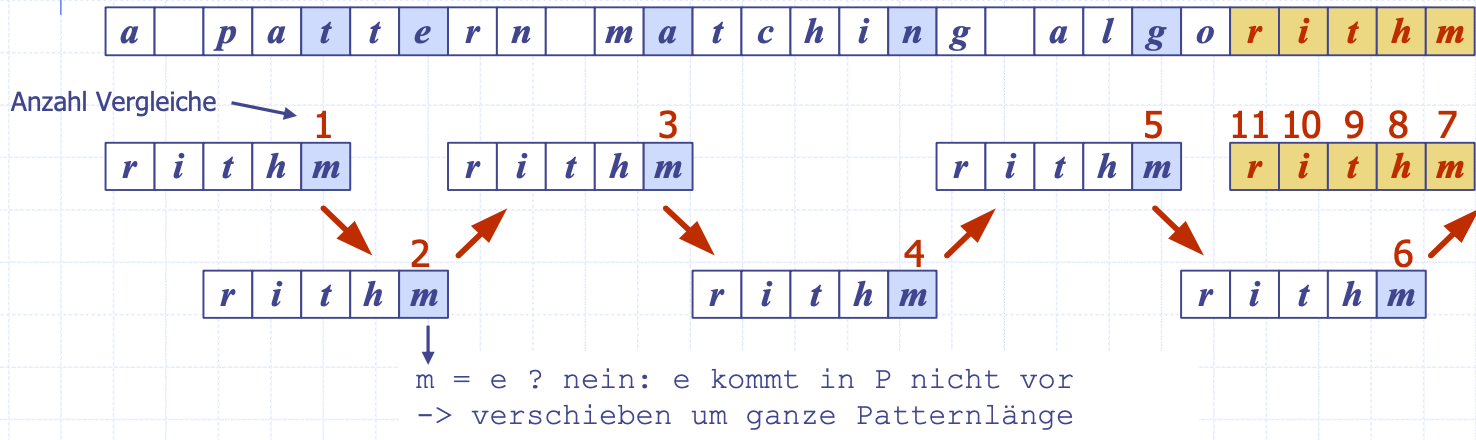
\includegraphics[scale=.25]{graphic/08 PatternMatching/Boyer-Moore def.png}
\end{center}
\vspace{-8pt}
\subsubsection{Laufzeit}
\begin{itemize}
    \item benötigt O(n * m + s)
    \item Worst Case:
    \begin{itemize}
        \item T=aaa...a
        \item P=baaa
    \end{itemize}
    \item Worst-Case kommt vor allem bei Bild- und DNA- Sequenzen vor und ist bei Text unwahrscheinlich
    \item ist signifikant schneller als der Brute-Force Algorithmus (angewandt auf Textanalysen)
\end{itemize}
\subsubsection{Algorithmus}
\begin{enumerate}
    \item Ist bereits das erste verglichene Textsymbol ein Symbol, das im Muster überhaupt nicht vorkommt, so kann das Muster um m Positionen hinter dieses Symbol weitergeschoben werden
    \item Falls eine Ungleichheit auftritt, das fehlerhafte Zeichen aber an anderer Stelle im Muster vorkommt, dann kann das Muster nur so weit geschoben werden, bis dieses Vorkommen ("die andere Stelle") auf das Textsymbol ausgerichtet ist
    \item Ergibt es eine negative Verschiebung, schiebe stattdessen um 1
\end{enumerate}
\subsection{Last-Occurrence Funktion}
Boyer-Moore's Algorithmus analysiert zuerst das Pattern P und das Alphabet $\Sigma$, um die last-occurrence Funktion L aufzubauen.\\
Diese bildet $\Sigma$ auf Integers ab, wobei L(c) wie folgt definiert ist:
\begin{itemize}
    \item $ L: \Sigma \rightarrow lN_0 \cup {-1}$
    \item $L: c \rightarrow L(c) =max_i {i|P[i]=c}$ falls c in P vorkommt, sonst -1
\end{itemize}
\begin{center}
    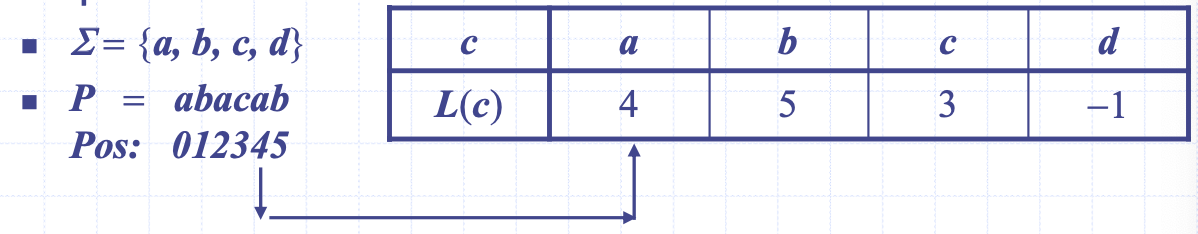
\includegraphics[scale=.28]{graphic/08 PatternMatching/Last-Occurrence.png}
\end{center}
\begin{itemize}
    \item Die Funktion L(c) lässt sich darstellen als ein Array, dessen Indices durch numerische Werte des Alphabets gegeben sind.
    \item Die Funktion lässt sich in O(m + s) berechnen, wobei m die Länge von P und s die Anzahl Zeichen in $\Sigma$ ist.
\end{itemize}
\subsubsection{Berechnung der Verschiebung}

\begin{itemize}
    \item Fall 1: Zeichen T[i] kommt im Pattern vor (last(T[i]> -1))
    \begin{itemize}
        \item Verschieben bis zum letzten Auftreten des Zeichens im Pattern
        \item Berechnung: i = i + m - (last(T[i]) + 1)
    \end{itemize}
    \item Fall 2: Zeichen kommt im Pattern vor, ist aber bereits vorhanden
    \begin{itemize}
        \item Pattern wird nach eine Stelle nach vorne verschoben
        \item i = i + m - j
    \end{itemize}
\end{itemize}

\paragraph{Boyer-Moore Algorithmus}

\textbf{1. "Last-Occurrence" - Funktion L(c) bestimmen}\\

\textbf{Spalte c:} Alle Buchstaben, die im Text vorkommen\\
\textbf{Spalte L(c):} falls im Pattern: letzte Position\\ 
\textbf{Spalte L(c):} falls nicht im Pattern: -1 \\

\textbf{2. Vergleichen}\\
Immer der hinterste Buchstaben des Patterns wird mit Text verglichen!\\

\textbf{3. Missmatch}\\
\begin{tabular}[]{p{2cm} p{3.8cm}}
    Buchstabe im Text & Ausrichten auf letztes Element\\
                      & bei negativer Verschiebung $\rightarrow$ 1 nach rechts\\
    \hline
    Buchstabe kommt \underline{nicht} im Text vor & Verschieben um ganze Patternlänge
\end{tabular}

\vfill
$ $
\columnbreak










\subsection{Knuth-Morris-Pratt (KMP) Algorithmus}
\subsubsection{Definition}
\begin{itemize}
    \item vergleicht das Muster gegen den Text von links-nach-rechts
    \item intelligenter als der Brute-Force
    \item Bei Nichtübereinstimmung: was ist das Maximum um das Muster zu verschieben? $\rightarrow$ längste Präfix von P[0..j] gleichzeitig Suffix von P[1..j] ist.
\end{itemize}
\vspace{-8pt}
\begin{center}
    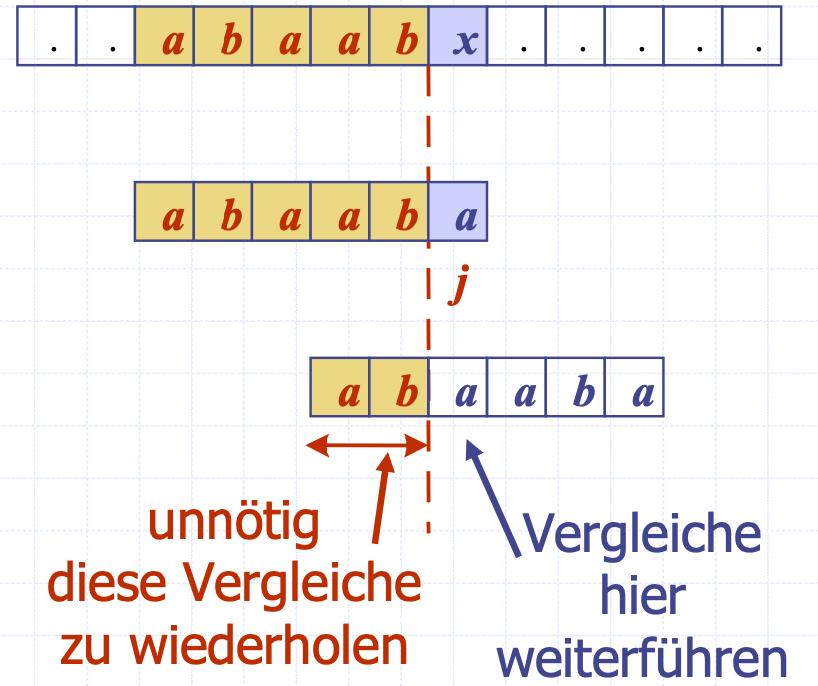
\includegraphics[scale=.2]{graphic/08 PatternMatching/KMP def.png}
\end{center}
\vspace{-8pt}
\subsubsection{Laufzeit}
\begin{itemize}
    \item failure function kann als Array dargestellt werden, in O(m) Zeit
\end{itemize}
\subsubsection{KMP Fehl-Funktion}
\begin{itemize}
    \item Vorlaufsphase sucht Algorithmus Übereinstimmungen von Präfixes des Musters im Muster selbst
    \item Die failure function F(j) ist definiert als die Grösse des längsten Präfixes von P[0..j] , so dass dieser auch Suffix von P[1..j] ist.
    \item KMP modifiziert den Brute-Force Algorithmus so, dass bei einer Differenz $P[j] \neq T[i]$ der Index j gesetzt wird mit: $ j \leftarrow F(j-1)$
\end{itemize}
\vspace{-8pt}
\begin{center}
    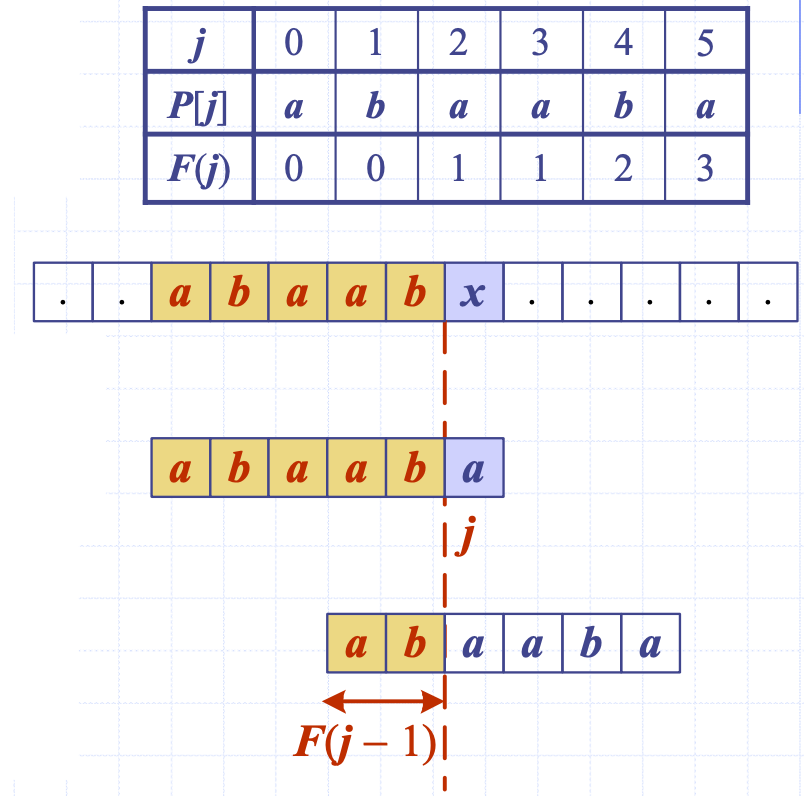
\includegraphics[scale=.2]{graphic/08 PatternMatching/KMP Fehl.png}
\end{center}
\vspace{-8pt}
\begin{lstlisting}
Algorithm failureFunction(P)
    F[0] <-- 0
    i <-- 1
    j <-- 0
    while i < m
        if P[i] == P[j]
        // we have matched j+1 chars
        F[i] <-- j+1
        i <-- i + 1
        j <-- j + 1
    else if j > 0
        // use failure function to shift P
        j <-- F[j-1]
    else
        F[i] <-- 0 // No match
        i <-- i + 1
\end{lstlisting}
\vspace{-8pt}
\begin{center}
    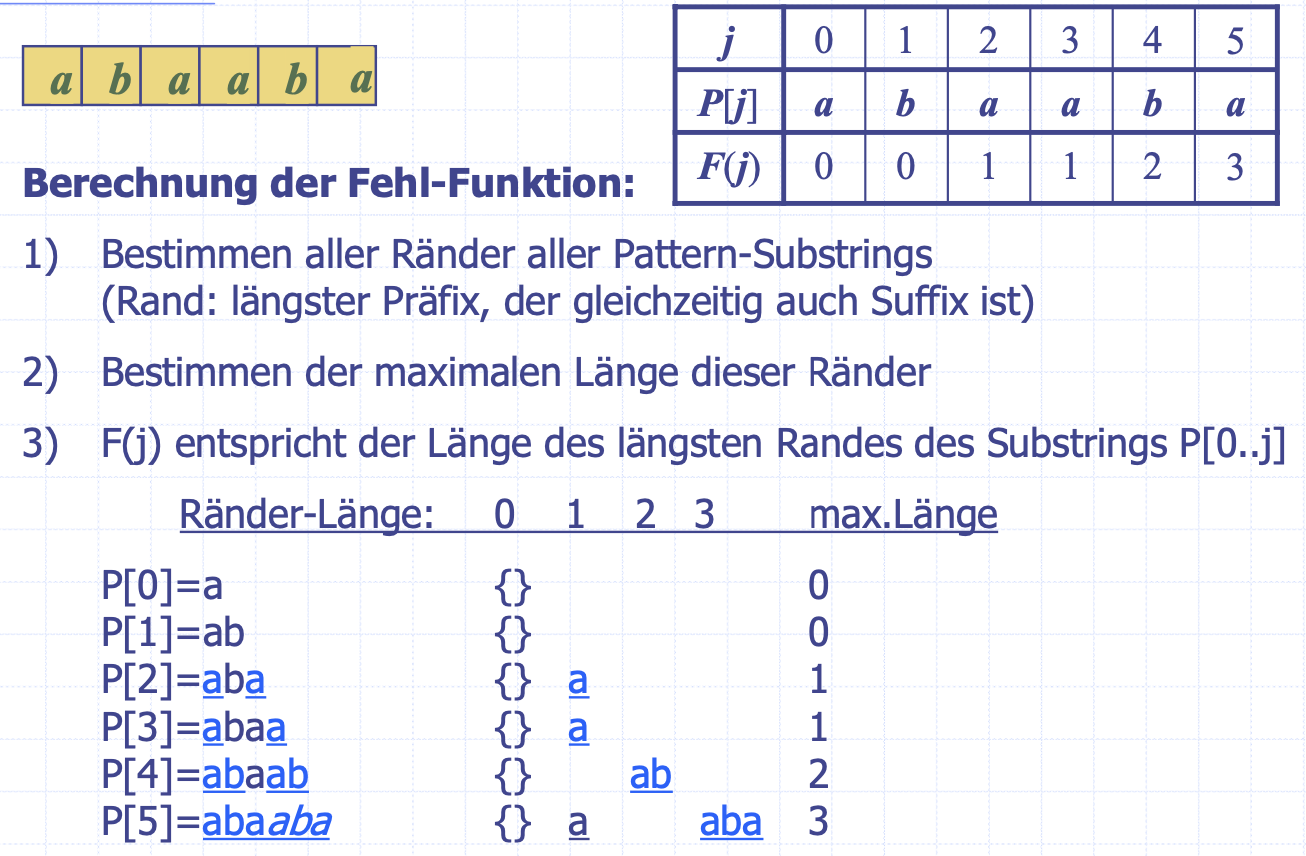
\includegraphics[scale=.25]{graphic/08 PatternMatching/KMP Fehl2.png}
\end{center}
\vspace{-8pt}

\subsubsection{Algorithmus}
Bei jeder Iteration der while- Schleife wird entweder:
\begin{itemize}
    \item i um eines erhöht
    \item Oder die Verschiebung i-j nimmt um mindestens 1 zu (F(j - 1) < j)
\end{itemize}
\begin{lstlisting}
Algorithm KMPMatch(T, P)
    F <-- failureFunction(P)
    i <-- 0
    j <-- 0
    while i < n
        if T[i] == P[j]
            if j == m -1
                return i - m + 1 // Match
            else
                i <-- i + 1
                j <-- j + 1
        else
            if j > 0
                j <-- F[j-1]
            else
                i <-- i + 1
    return -1 // No match
\end{lstlisting}
\vspace{-8pt}
\begin{center}
    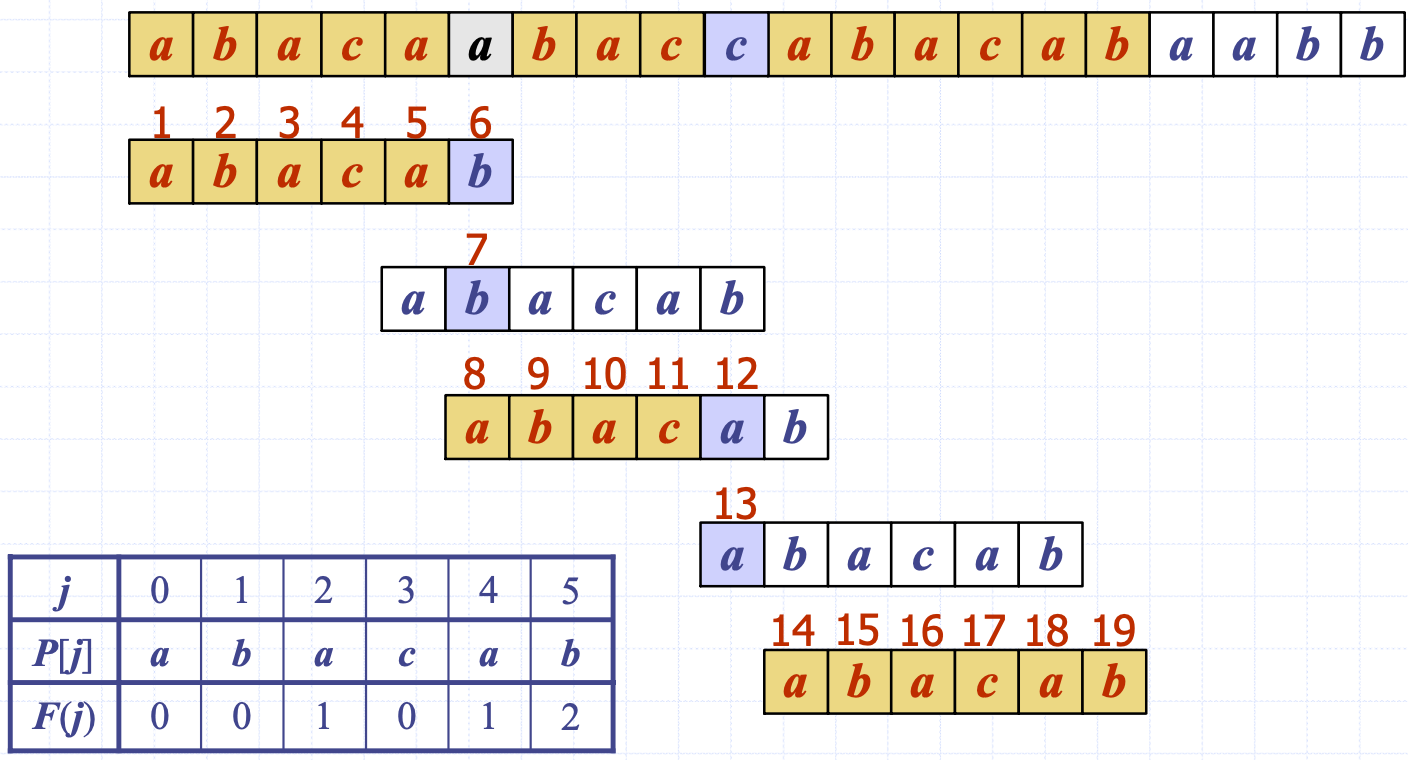
\includegraphics[scale=.2]{graphic/08 PatternMatching/KMP.png}
\end{center}
\vspace{-8pt}

\paragraph{Knuth-Morris-Pratt (KMP)}
\textbf{1. KMP Fehl-Funktion F(j) bestimmen}\\

\textbf{Spalte P(j):} Pattern selbst\\
\textbf{Spalte F(j):} Maximale Ränder Länge
\begin{center}
    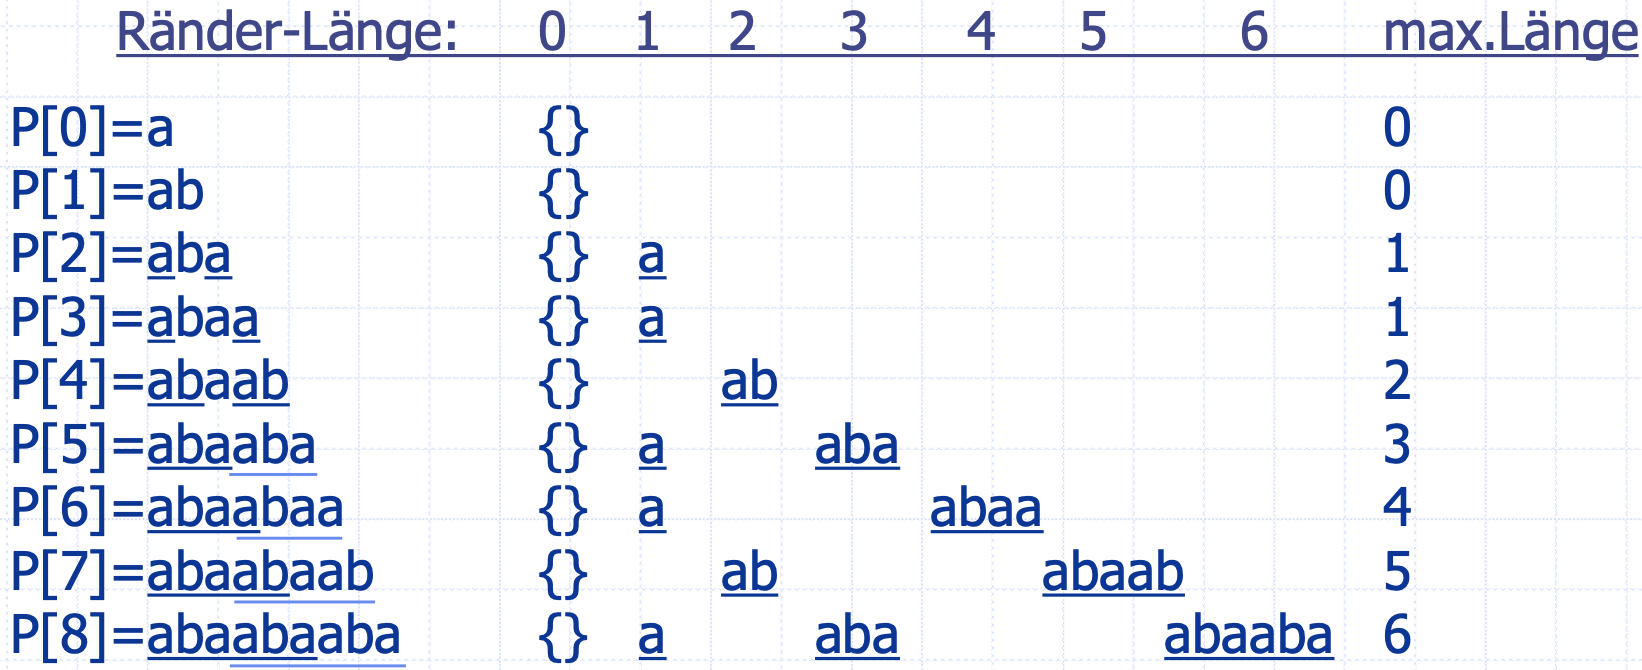
\includegraphics[scale=.2]{graphic/08 PatternMatching/KMP Fehl3.png}
\end{center}

\textbf{2. Vergleichen}\\
Immer der vordeste Buchstaben des Patterns wird mit Text verglichen!\\

\textbf{3. Missmatch}
\begin{center}
    \begin{tabular}[]{p{2cm} p{4cm}}
        Fehler ist 1. Buchstabe        & Verschiebung um 1 nach rechts\\
        \hline
         Fehler ist \underline{nicht} 1. Buchstabe & Fehlgeschlagener (Pattern-) Buchstabe im F(j) suchen\\
                & An Position F(j-1) verschieben (direkt unten) 
    \end{tabular}
\end{center}

\vfill
$ $

\newpage
    \section{Tries}

\subsection{Preprocessing Strings}
\begin{itemize}
    \item Durch Vorverarbeitung des Musters wird eine Geschwindigkeitsverbesserung beim Suchen erzielt
    \item Nach Vorverarbeitung des Musters erzielt der KMP Algorithmus eine Geschwindigkeit, die proportional zur Text-Grösse ist
    \item Ist der Text gross, unveränderlich und wird oft durchsucht (z.B. das Werk von Shakespeare): man könnte anstelle des Musters den Text vorverarbeiten
    \item Trie ist eine kompakte Datenstruktur für die Repräsentation einer Menge von Strings, wie z.B alle Wörter eines Textes
    \item Tries erlauben Pattern Matching mit einer Geschwindigkeit welche proportional zur Grösse des Patterns ist
\end{itemize}


\subsection{Standard Tries}
für eine Menge von Strings S ist ein geordneter Baum, so dass:
\begin{itemize}
    \item jeder ausser dem Wurzel-Knoten ein Zeichen hat
    \item die Pfade von den externen Knoten zur Wurzel die Strings von S beinhalten
\end{itemize}
\vspace{-8pt}
\begin{center}
    \includegraphics[scale=.3]{graphic/09 Tries/Standard Tries.png}
\end{center}
\vspace{-10pt}
\subsubsection{Laufzeit}
\begin{itemize}
    \item benötigt O(n) Speicher
    \item Suchen, Einfügen und Löschen in O(dm)
    \begin{itemize}
        \item n = totale Länge der Strings in S
        \item m = Länge des String-Parameters der Operation
        \item d = Grösse des Alphabets
    \end{itemize}
\end{itemize}
\subsubsection{Suche}
\begin{center}
    \includegraphics[scale=.25]{graphic/09 Tries/suche.png}
\end{center}
\vspace{-8pt}


\subsubsection{Komprimierte Tries}
\begin{itemize}
    \item wird von einem Standard-Trie hergeleitet
    \item Komprimierung von Pfaden von redundanten Knoten
\end{itemize}
\vspace{-8pt}
\begin{multicols}{2}
Standard-Trie:
\begin{center}
    \includegraphics[scale=.165]{graphic/09 Tries/unkomprimiert.png}
\end{center}
    \columnbreak
Komprimierter Trie:
\begin{center}
    \includegraphics[scale=.23]{graphic/09 Tries/komprimiert.png}
\end{center}
\end{multicols}
\vspace{-8pt}
\subsubsection{Kompakte Repräsentation}
\begin{itemize}
    \item Knoten speichert Indizes anstelle von Substrings
    \item Benötigt O(s) Speicher, wobei s die Anzahl Strings im Array ist
    \item Dient als eine Hilfs-Index-Struktur
\end{itemize}
\vspace{-8pt}
\begin{center}
    \includegraphics[scale=0.28]{graphic/09 Tries/Kompakte_Repräsentation.png}
\end{center}
\vspace{-8pt}



\subsection{Suffix Trie}
\begin{itemize}
    \item Suffix-Trie eines Strings X ist der komprimierte Trie von allen Suffixen von X
\end{itemize}
\vspace{-8pt}
\begin{center}
    \includegraphics[scale=0.25]{graphic/09 Tries/Suffix.png}
\end{center}
\vspace{-8pt}
\subsubsection{Laufzeit}
\begin{itemize}
    \item benötigt O(n) Speicher
    \item Pattern Matching in X in O(dm)
    \item in O(n) Zeit erstellt werden
    \item X = Strings
    \item n = Länge von X
    \item d = Grösse des Alphabet
    \item m = Länge des Patterns
\end{itemize}

\newpage
    \section{Dynamic Programming}

\subsection{Rucksack-Problem}
Gegeben:
\begin{itemize}
    \item n Gegenstände mit einem bestimmten Gewicht und Wert
    \item Rucksack mit einer bestimmten Gewichts-Kapazität
\end{itemize}
Gesucht:
\begin{itemize}
    \item Füllung des Rucksacks, so dass der Wert der Gegenstände maximal ist
\end{itemize}

\subsubsection{Versuch mit Brute Force}
\begin{itemize}
    \item Versuche alle möglichen Varianten
    \item Beachte nur wenn maximale Gewicht nicht überschreiten
\end{itemize}
$\rightarrow$ Laufzeit exponentiell: $O(2^n)$

\subsubsection{Versuch mit Greedy-Algorithmus}
\begin{itemize}
    \item nimm wiederholend den Gegenstand mit grössten Verhältnis von Wert/Gewicht
    \item Nicht optimales Ergebnis!
\end{itemize}
\subsubsection{Versuch mit Dynamische Programmierung (Subproblemen)}
\begin{itemize}
    \item Optimale Subprobleme bottom-up konstruieren
    \item Probleme der Länge 1 sind einfach $\rightarrow$ beginnen
    \item Dann Subprobleme der Längen 2,3,...
    \item Subprobleme beim Rucksack:
    \begin{itemize}
        \item 1..4 Gegenstände
        \item 1..5 kg maximales Gewicht
    \end{itemize}
\end{itemize}
\vspace{-8pt}
\begin{center}
    \includegraphics[scale=.2]{graphic/10 DynamicProgramming/Dynamische Programmierung.png}
    \includegraphics[scale=.2]{graphic/10 DynamicProgramming/Dynamische Programmierung2.png}
\end{center}
\vspace{-8pt}

\subsection{Technik der dynamischen Programmierung}
\begin{itemize}
    \item Anwendbar auf Probleme welche anfänglich sehr grosse Laufzeit zu benötigen
    \item Voraussetzung:
    \begin{itemize}
        \item \textbf{Einfache Subprobleme:} Subprobleme können durch wenigen Variablen ausgedrückt werden
        \item \textbf{Subproblem-Optimierung:} globale Optimum kann durch optimale Subprobleme ausgedrückt werden
        \item \textbf{Subprobleme überlappen: }Subprobleme sind nicht unabhängig, sie überlappen
    \end{itemize}
\end{itemize}

\subsection{Subsequenzen}
\begin{itemize}
    \item Nicht dasselbe wie ein Substring
    \item Beispiel: ABCDEFGHIJK
    \begin{itemize}
        \item Subsequenz: ACEGIJK
        \item Subsequenz: DFGHK
        \item Nicht Subsequenz: DAGH
    \end{itemize}
\end{itemize}

\subsection{Längste gemeinsame Subsequenz (LCS)}
\begin{itemize}
    \item Gegeben die beiden Strings X und Y
    \item finde die längste Subsequenz welche in X sowie auch in Y enthalten ist
    \item Beispiel: ABCDEFG und XZACKDFWGH haben ACDFG als längste gem. SubSeq.
\end{itemize}
\subsubsection{Brute-Force}
\begin{itemize}
    \item Aufzählung aller Subsequenzen von X
    \item Testen welche ebenfalls Subsequenzen von Y sind
    \item längste Subsequenz als Resultat wählen
    \item exponentieller Algorithmus! $\rightarrow$ $O(n^2)$
\end{itemize}
\subsubsection{dynamischer Programmierung}
\begin{itemize}
    \item Definiere L[i,j] als Länge der längsten gemeinsamen Subsequenz von X[0..i] and Y[0..j]
    \item Erlaube -1 als Index, so dass L[-1,k] = 0 and L[k,-1]=0
    \item Definiere L[i,j] folgendermassen:
    \begin{itemize}
        \item wenn $xi = yj$, dann L[i,j] = L[i-1,j-1] + 1 (Übereinstimmung)
        \item wenn $xi \neq yj$, dann L[i,j] = max{L[i-1,j], L[i,j-1]} (keine Übereinstimmung)
    \end{itemize}
\end{itemize}
\vspace{-8pt}
\begin{center}
    \includegraphics[scale=.2]{graphic/10 DynamicProgramming/Versuch mit dynamischer Programmierung.png}
    \includegraphics[scale=.2]{graphic/10 DynamicProgramming/Versuch mit dynamischer Programmierung2.png}
\end{center}
\vspace{-8pt}

\begin{lstlisting}
Algorithmus LCS(X,Y):
    Input: Strings X,Y with n,m Elements
    Output: array L[i,j]
    for i=1 to n-1 do
        L[i,-1] = 0
    for j=0 to m-1 do
        L[-1, j] = 0
    for i=0 to n-1 do
        for j=0 to m-1 do
            if x_i = y_i then
                L[i,j] = L[i-1, j-1] + 1
            elseL[i,j] = max{L[i-1,j],L[i,j-1]}
    return array L
\end{lstlisting}

\subsubsection{Laufzeit}
\begin{itemize}
    \item äusserer Loop iteriert n mal
    \item innerer Loop iteriert m mal
    \item konstanter Aufwand innerhalb jeder Iteration des inneren Loops
    \item Somit ist die totale Laufzeit: O(nm)
\end{itemize}

\subsubsection{Auslesen der LCS}
\begin{center}
    \includegraphics[scale=.2]{graphic/10 DynamicProgramming/Auslesen der LCS.png}
\end{center}

\newpage
    \section{Graphen}
Ein Graph ist ein Paar (V, E), wobei:
\begin{itemize}
    \item V ist ein Set von Vertizes (Knoten)
    \item E ist eine Collection von Vertizes-Paaren, Kanten (Edge)
    \item Vertizes und Kanten sind Positionen und speichern Elemente
\end{itemize}

\subsection{Kanten-Typen}
\begin{itemize}
    \item gerichtete Kanten
    \begin{itemize}
        \item geordnetes Paar von Vertizes (u,v)
        \item erster Vertex u entspricht dem Ursprung
        \item zweiter Vertex v entspricht dem Ziel
        \item z.B. Flug
    \end{itemize}
    \item ungerichtete Kanten
    \begin{itemize}
        \item ungeordnetes Vertizes-Paar (u,v)
        \item z.B. Flugroute
    \end{itemize}
    \item gerichteter Graph
    \begin{itemize}
        \item alle Kanten sind gerichtet
        \item z.B. Flugplan
    \end{itemize}
    \item ungerichter Graph
    \begin{itemize}
        \item alle Kanten sind ungerichtet
        \item z.B. Flugrouten-Plan
    \end{itemize}
\end{itemize}


\subsection{Laufzeit}
\begin{center}
    \includegraphics[scale=.2]{graphic/11 Graph/Laufzeit.png}
\end{center}
\vspace{-8pt}


\subsection{Terminologie}
\begin{itemize}
    \item Kanten sind \textbf{inzident} (enden) an einem Vertex
    \item \textbf{Adjazente} (benachbarte) Vertizes
    \item \textbf{Grad (Degree)} eines Vertex: Anzahl inzidenter Kanten
    \item \textbf{Parallele Kanten}
    \item \textbf{Schleife}
    \item \textbf{Pfad}
    \begin{itemize}
        \item Sequenz von alternierenden Vertizes und Kanten
        \item beginnt mit einem Vertex
        \item endet mit einem Vertex
        \item jede Kante beginnt und endet an einem ihrer Endpunkte
    \end{itemize}
    \item \textbf{Einfacher Pfad}
    \begin{itemize}
        \item ein Pfad, so dass alle seine Vertizes und Kanten unterschiedlich sind
    \end{itemize}
    \item \textbf{Zyklus}
    \begin{itemize}
        \item zirkuläre Sequenz alternierender Vertizes und Kanten
    \end{itemize}
    \item \textbf{Einfacher Zyklus}
    \begin{itemize}
        \item ein Zyklus, so dass alle seine Vertizes und Kanten unterschiedlich sind
    \end{itemize}
\end{itemize}


\subsection{Eigenschaften}
\begin{itemize}
    \item \textbf{Notation:}
    \begin{itemize}
        \item n = Anzahl Vertizes
        \item m = Anzahl Kanten
        \item deg(v) = Grad von Vertex v
    \end{itemize}
    \item \textbf{Eigenschaft 1:}
    \begin{itemize}
        \item $\Sigma_v deg(v) = 2m$
        \item Beweis: jede Kante wird zweimal gezählt
    \end{itemize}
    \item \textbf{Eigenschaft 2:}
     \begin{itemize}
        \item In einem ungerichteten Graphen ohne Schleifen und ohne parallele Kanten gilt:
        \item m $\leqslant$  n (n - 1) / 2
        \item entspricht einem ungerichteten, einfachen Graphen
        \item Beweis: jeder Vertex besitzt einen Grad von höchstens (n - 1)
     \end{itemize}
\end{itemize}

\vspace{-8pt}
\begin{center}
    \includegraphics[scale=.25]{graphic/11 Graph/Eigenschaften.png}
\end{center}
\vspace{-8pt}


\subsection{Haupt-Methoden}
\begin{center}
    \includegraphics[scale=.25]{graphic/11 Graph/Methoden.png}
\end{center}
\vspace{-8pt}


\subsection{Struktur}

\subsubsection{Kanten-Listen}

\begin{center}
    \includegraphics[scale=.23]{graphic/11 Graph/Kanten-Listen.png}
\end{center}
\vspace{-8pt}

\subsubsection{Adjazenz-Listen}
\begin{center}
    \includegraphics[scale=.23]{graphic/11 Graph/Adjazenz-Listen.png}
\end{center}
\vspace{-8pt}


\subsubsection{Adjazenz-Matrix}
\begin{center}
    \includegraphics[scale=.23]{graphic/11 Graph/Adjazenz-Matrix.png}
\end{center}
\vspace{-8pt}


\subsection{Subgraphen}
\begin{center}
    \includegraphics[scale=.23]{graphic/11 Graph/Subgraphen.png}
\end{center}
\vspace{-8pt}

\subsection{Connectivity}
\begin{center}
    \includegraphics[scale=.2]{graphic/11 Graph/Connectivity.png}
\end{center}
\vspace{-8pt}


\subsection{Bäume und Wälder}
\begin{center}
    \includegraphics[scale=.23]{graphic/11 Graph/Bäume und Wälder1.png}
\end{center}
\vspace{-8pt}


\subsection{Spanning Trees und Wälder}
\begin{center}
    \includegraphics[scale=.25]{graphic/11 Graph/Bäume und Wälder2.png}
\end{center}
\vspace{-8pt}

\vfill
$ $
\columnbreak

\paragraph{Graph Implementation}

\begin{lstlisting}
public class KantenListenGraph {
    private DoubleLinkedPosition<Vertex> vSeqHead;
    private DoubleLinkedPosition<Edge> eSeqHead;
    
    public Vertex insertVertex(Object o) {
        vSeqHead = new DoubleLinkedPosition<Vertex>(vSeqHead);
        Vertex vertex = new Vertex(o, vSeqHead);
        return vertex;
    }
    
    public Edge insertEdge(Vertex v, Vertex w, Object o) {
        Vertex[] endVertices = {v, w};
        eSeqHead = new DoubleLinkedPosition<Edge>(eSeqHead);
        Edge edge = new Edge(o, endVertices, eSeqHead);
        return edge;
    }

public class Vertex {
    private Object object;
    protected DoubleLinkedPosition<Vertex> position;
    
    public Vertex(Object o, DoubleLinkedPosition<Vertex> position) {
        this.object = o;
        this.position = position;
        position.element = this;
  }

public class Edge {
    private Object object;
    private Vertex[] vertices;
    protected DoubleLinkedPosition<Edge> position;
    
    public Edge(Object o, Vertex[] vertices, DoubleLinkedPosition<Edge> position) {
        this.object = o;
        this.vertices = vertices;
        this.position = position;
        position.element = this;
}

public class DoubleLinkedPosition<E> {
    protected DoubleLinkedPosition<E> previous;
    protected DoubleLinkedPosition<E> next;
    protected E element;
    
    DoubleLinkedPosition(DoubleLinkedPosition<E> next) {
        this.next = next;
        if (next != null) {
            next.previous = this;
        }
    }
}
\end{lstlisting}


\newpage  
    \section{Depth-First Search (DFS) (Tiefensuche)}

\subsection{Definition}
\begin{itemize}
    \item ist allgemeine Technik für die Traversierung eines Graphen
    \item Eine DFS Traversierung eines Graphen G
    \begin{itemize}
        \item besucht alle Vertizes und Kanten von G
        \item bestimmt, ob G verbunden ist
        \item berechnet / bestimmt die verbundenen Komponenten von G
        \item berechnet einen aufspannenden Wald von G
    \end{itemize}
    \item DFS kann man auch erweitern, um andere Graphenprobleme zu lösen
    \item Depth-First Search entspricht in etwa der Euler-Tour bei binären Bäumen
\end{itemize}


\subsection{Laufzeit}
\begin{itemize}
    \item DFS auf einem Graphen mit n Vertizes und m Kanten benötigt O(n + m) Zeit
    \item Setzen/Lesen eines Vertex-/Kanten-Labels benötigt O(1) Zeit
    \item Jeder Vertex wird zweimal markiert:
    \begin{itemize}
        \item zuerst als UNEXPLORED
        \item dann als VISITED
    \end{itemize}
    \item Jede Kante wird zweimal markiert:
    \begin{itemize}
        \item zuerst als UNEXPLORED
        \item dann als DISCOVERY oder BACK
    \end{itemize}
    \item Die Methode incidentEdges() wird pro Vertex einmal aufgerufen
\end{itemize}


\subsection{Algorithmus}
\begin{center}
    \includegraphics[scale=.4]{graphic/12 DFS/Algorithmus.png}
\end{center}
\vspace{-8pt}


\subsection{Beispiel}
\begin{center}
    \includegraphics[scale=.4]{graphic/12 DFS/Beispiel.png}
\end{center}
\vspace{-8pt}


\subsection{Labyrinth}
Der DFS Algorithmus ähnelt der klassischen Strategie zur Erkundung eines Labyrinths:
\begin{itemize}
    \item markieren jede besuchte Kreuzung, Ecke und Sackgasse (Vertex)
    \item wir markieren jeden besuchten Korridor (Kante)
    \item notieren den Rückweg zum Eingang (Start Vertex) ($\rightarrow$ Rekursion auf dem Stack)
\end{itemize}


\subsection{Eigenschaften}
\begin{itemize}
    \item \textbf{Eigenschaft 1:} DFS(G, v) besucht alle Vertizes und Kanten in der verbundenen Komponente von G beginnend bei v
    \item \textbf{Eigenschaft 2:} die von DFS(G, v) markierten, besuchten Kanten bilden einen aufspannenden Baum für die verbundene Komponente von G beginnend bei v
\end{itemize}

\subsection{Pfade finden}
\begin{itemize}
    \item DFS Algorithmus spezialisieren, um einen Pfad zwischen zwei gegebenen Vertizes u und z zu finden.
    \item zuerst DFS(G, u) aufrufen mit u als Startvertex
    \item mithilfe eines Stacks S den Pfad merken zwischen dem Startvertex und dem aktuellen Vertex
    \item sobald Zielvertex z gefunden, Pfad mithilfe des Stacks ausgeben
\end{itemize}
\vspace{-8pt}
\begin{center}
    \includegraphics[scale=.3]{graphic/12 DFS/Pfade finden.png}
\end{center}
\vspace{-8pt}


\subsection{Zyklen finden}
\begin{itemize}
    \item DFS Algorithmus spezialisieren, um einfache Zyklen zu finden
    \item mithilfe eines Stacks S den Pfad merken zwischen Startvertex und aktuellen Vertex
    \item sobald auf eine Back- Edge (v, w) treffen, Zyklus als Teil des Stacks aus:
    \item vom obersten Stackelement bis zum Vertex w.
\end{itemize}
\vspace{-8pt}
\begin{center}
    \includegraphics[scale=.3]{graphic/12 DFS/Zyklen finden.png}
\end{center}
\vspace{-8pt}

\vfill
$ $
\columnbreak
\paragraph{Tiefensuche}
\begin{center}
    \includegraphics[scale=.3]{12 DFS/tiefensuche.png}
\end{center}

\paragraph{Gerichtete Tiefensuche Typen}
\begin{center}
    \includegraphics[scale=.33]{12 DFS/gerichtete_tiefensuche.png}
\end{center}


\paragraph{Gerichtete Tiefensuche Algorithmus}
\begin{enumerate}
    \item Starte bei 1 respektive A
    \item Gehe zum nächstliegenden Buchstaben / Zahl
    \item Solange in Tiefe suchen, bis nicht mehr weiter geht
    \item Zurück, bis wieder weitergesucht werden kann
\end{enumerate}
\begin{center}
    \includegraphics[scale=.33]{12 DFS/gerichtete_tiefensuche_alg.png}
\end{center}


\newpage
    \section{Breadth-First Search (BFS) (Breitensuche)}
\begin{itemize}
    \item eine generelle Technik für die Traversierung eines Graphen
    \item besucht alle Vertizes und alle Kanten von G
    \item bestimmt, ob G verbunden ist
    \item berechnet / bestimmt die verbundene Komponenten von G
    \item berechnet einen aufspannenden Wald von G
    \item kann man auch erweitern, um andere Graphenprobleme zu lösen
    \begin{itemize}
        \item Finden und Ausgeben eines Pfades mit einer minimalen Anzahl Kanten zwischen zwei gegebenen Vertizes
        \item Finden von einfachen Zyklen
    \end{itemize}
\end{itemize}


\subsection{Laufzeit}
\begin{itemize}
    \item auf einem Graphen mit n Vertizes und m Kanten benötigt O(n + m) Zeit
    \item Setzen/Lesen eines Vertex-/Kanten-Labels benötigt O(1) Zeit
    \item Jeder Vertex wird zweifach markiert
    \begin{itemize}
        \item einmal als UNEXPLORED
        \item einmal als VISITED
    \end{itemize}
    \item Jede Kante wird zweifach markiert
    \begin{itemize}
        \item einmal als UNEXPLORED
        \item einmal als DISCOVERY oder CROSS
    \end{itemize}
    \item Die Methode incidentEdges() wird einmal pro Vertex aufgerufen
\end{itemize}


\subsection{Algorithmus}
\begin{center}
    \includegraphics[scale=.25]{graphic/13 BFS/Algorithmus.png}
\end{center}
\vspace{-8pt}




\subsection{Beispiel}
\begin{center}
    \includegraphics[scale=.3]{graphic/13 BFS/bsp.png}
\end{center}
\vspace{-8pt}

\subsection{Eigenschaften}
\begin{itemize}
    \item \textbf{Notation:}
    \begin{itemize}
        \item s = Start-Vertex
        \item $G_s$: verbundene Komponente von s
    \end{itemize}
    \item \textbf{Eigenschaft 1:}
    \begin{itemize}
        \item BFS(G, s) besucht alle Vertizes und Kanten in $G_s$
    \end{itemize}
    \item \textbf{Eigenschaft 2:}
    \begin{itemize}
        \item Die Discovery-Kanten von BFS(G, s) bilden einen aufspannenden Baum $T_s$ von $G_s$
    \end{itemize}
    \item \textbf{Eigenschaft 2:}\\
    für jeden Vertex v in Li gilt:
    \begin{itemize}
        \item der Pfad in $T_s$ von s nach v besitzt i Kanten
        \item Jeder Pfad von s nach v in $G_s$ besitzt mindestens i Kanten
    \end{itemize}
\end{itemize}

\subsection{Anwendungen}
\begin{itemize}
    \item bestimmen der verbundenen Komponenten von G
    \item bestimmen eines aufspannenden Waldes von G
    \item bestimmen eines einfachen Zyklus in G, oder bestimmen, ob G ein Wald ist
    \item bei zwei gegebenen Vertizes von G: finden eines Pfades in G zwischen den beiden Vertizes mit minimaler Anzahl Kanten oder bestimmen, ob ein solcher Pfad existiert
\end{itemize}
\subsection{DFS vs. BFS}
\begin{center}
    \includegraphics[scale=.25]{graphic/13 BFS/DFS vs. BFS1.png}
    \includegraphics[scale=.25]{graphic/13 BFS/DFS vs. BFS2.png}
\end{center}
\vspace{-8pt}

\vfill
$ $
\columnbreak
\paragraph{Breitensuche}
\begin{center}
    \includegraphics[scale=.25]{graphic/13 BFS/breitensuche.png}
\end{center}

\paragraph{Kürzester Pfad}
\begin{enumerate}
    \item Start Bei A
    \item Alle Distanzen = $\infty$, ausser direkt verbundene $\rightarrow$ Einzeichnen!
    \item Kürzeste Distanz verbinden (hier B)
    \item neue Distanzen einfügen
    \item Ab Schritt 3 wiederholen
\end{enumerate}
\begin{center}
    \includegraphics[scale=.25]{13 BFS/Kürzester Pfad.png}
\end{center}
\newpage
    \section{Gerichtete Graphen}
\begin{itemize}
    \item Graph, dessen Kanten alle gerichtet sind
    \item Digraph ist: G = (V,E)
    \item Wenn G einfach ist: m < n(n-1)
    \item Wenn In- und Out-Kanten in separaten Adjazenz- Listen sind: Laufzeit für Zugriff auf In- und Out-Kanten proportional zur Grösse der Listen
\end{itemize}

\subsection{Gerichtete Tiefensuche}
\begin{itemize}
    \item DFS und BFS für Digraphen spezialisieren, indem Kanten nur entlang ihrer Richtung traversiert werden
    \item Im gerichteten DFS-Algorithmus haben wir vier Typen von Kanten:
\end{itemize}
\vspace{-8pt}
\begin{center}
    \includegraphics[scale=.28]{graphic/14 Digraphs/Gerichtete Tiefensuche.png}
\end{center}
\vspace{-8pt}
Eine gerichtete Tiefensuche beginnt bei einem Vertex s und bestimmt die Vertizes, welche von s aus erreichbar sind

\subsection{Erreichbarkeit}
DFS Baum mit Wurzel v : Vertizes erreichbar von v durch gerichtete Pfade
\vspace{-8pt}
\begin{center}
    \includegraphics[scale=.22]{graphic/14 Digraphs/Erreichbarkeit.png}
\end{center}
\vspace{-8pt}

\subsection{Strong Connectivity}
Jeder Vertex kann alle anderen Vertizes erreichen
\subsubsection{Algorithmus}
\begin{itemize}
    \item Wähle einen Vertex v in G
    \item Führe eine Tiefensuche von v in G durch
    \begin{itemize}
        \item wenn es einen nicht besuchten Vertex w gibt: return false
    \end{itemize}
    \item G’ sei G mit umgekehrten Kanten (Richtungen)
    \item Führe eine Tiefensuche durch von v in G’
    \begin{itemize}
        \item wenn es einen nicht besuchten Vertex w gibt: return false
        \item sonst: return true //OK
    \end{itemize}
\end{itemize}
Laufzeit: O(n+m)

\subsection{Streng verbundene Komponenten}
\begin{itemize}
    \item Maximaler Subgraph, sodass jeder Vertex alle anderen Vertizes im Subgraph erreichen kann
    \item Laufzeit: O(n+m) mit Tiefensuche, ist aber komplizierter (ähnlich zu Biconnectivity)
\end{itemize}
\vspace{-8pt}
\begin{center}
    \includegraphics[scale=.2]{graphic/14 Digraphs/Streng verbundene Komponenten.png}
\end{center}
\vspace{-8pt}

\subsection{Transitiver Abschluss}
Laufzeit: O(n(n+m))
\vspace{-8pt}
\begin{center}
    \includegraphics[scale=.28]{graphic/14 Digraphs/Transitiver Abschluss.png}
\end{center}
\vspace{-8pt}

\subsection{Floyd-Warshall Algorithmus}

\begin{center}
    \includegraphics[scale=.22]{graphic/14 Digraphs/Floyd-Warshall Algorithmus.png}
    \includegraphics[scale=.28]{graphic/14 Digraphs/Floyd-Warshall Algorithmus2.png}
    \includegraphics[scale=.22]{graphic/14 Digraphs/Floyd-Warshall Algorithmus3.png}
\end{center}
\vspace{-8pt}

\subsection{DAG’s und topologische Ordnung}
\begin{itemize}
    \item gerichteter azyklischer Graph (Directed Acyclic Graph (DAG)) ist ein Digraph, der keine gerichtete Zyklen enthält
    \item Eine topologische Ordnung eines Digraphs ist definiert durch die Nummerierung: $v_1 , ..., v_n$ der Vertizes, sodass für jede Kante ($v_i , v_j$) gilt: i < j
\end{itemize}
\vspace{-8pt}
\begin{center}
    \includegraphics[scale=.25]{graphic/14 Digraphs/DAG.png}
\end{center}
\vspace{-8pt}
\subsubsection{Topologische Sortierung}
Laufzeit: O(n + m)
Nummeriere Vertizes, sodass für (u,v) in E gilt: u < v
\vspace{-8pt}
\begin{center}
    \includegraphics[scale=.28]{graphic/14 Digraphs/topologische Sortierung.png}
\end{center}
\vspace{-8pt}
\subsubsection{Topologische Sortierung mit Tiefensuche}
\begin{center}
    \includegraphics[scale=.28]{graphic/14 Digraphs/topologische Sortierung mit Tiefensuche.png}
\end{center}
\vspace{-8pt}

\newpage
    \section{Shortest Path Trees}

\subsection{Gewichtete Graphen}
\begin{itemize}
    \item jede Kante hat einen assoziierten nummerischen Wert (Gewicht)
    \item z.B. Distanzen, Kosten, etc. repräsentieren
\end{itemize}

\subsection{Kürzester Pfad}
\begin{itemize}
    \item Gegeben sei ein gewichteter Graph mit zwei Vertizes u und v.
    \item Wir möchten den Weg mit dem kleinsten totalen Gewicht zwischen u und v finden
    \item Die Länge des Pfades ist die Summe der Gewichte seiner Kanten
\end{itemize}
\subsubsection{Eigenschaften}
\begin{itemize}
    \item \textbf{Eigenschaft 1:} Ein Teilweg eines kürzesten Weges ist selbst auch ein kürzester Weg
    \item \textbf{Eigenschaft 2:} Es existiert ein Baum von kürzesten Wegen von einem Start-Vertex zu allen anderen Vertizes.
    \item \textbf{Eigenschaft 3:}Baum der kürzesten Wege von Providence
\end{itemize}

\subsection{Dijkstra’s Algorithmus}
\begin{itemize}
    \item Die Distanz eines Vertex v zu einem Vertex s ist die Länge des kürzesten Pfades zwischen s und v
    \item Dijkstra’s Algorithmus berechnet die Distanzen zu allen Vertizes von einem Start-Vertex s aus
\end{itemize}

\subsubsection{Ablauf}
\begin{itemize}
    \item bilden eine Wolke (Cloud) von Vertizes, beginnend mit s und fügen nach und nach alle Vertizes ein
    \item Mit jedem Vertex v speichern wir eine Eigenschaft d(v) welche die Distanz von v zu s im Untergraph (bestehend aus der Wolke und den Nachbar-Vertizes) angibt
    \item Bei jedem Schritt
    \begin{itemize}
        \item fügen der Wolke den Vertex u hinzu, welcher ausserhalb der Wolke ist und die kleinste Distanz d(u) aufweist
        \item aktualisieren die Distanzen von allen Nachbar-Vertizes von u
    \end{itemize}
\end{itemize}

\subsubsection{Laufzeit}
\begin{itemize}
    \item Methode incidentEdges wird für jeden Vertex einmal aufgerufen
    \item Wir setzen/lesen das Distanz- und das Locator-Label eines Vertex z O(deg(z)) mal
    \item Setzen/Lesen eines Labels braucht O(1) Zeit
    \item Jeder Vertex wird einmal in die Priority Queue eingefügt und einmal gelöscht, wobei jedes Einfügen und Löschen O(log n) Zeit benötigt
    \item Der Schlüssel eines Vertex w in der Priority Queue wird maximal deg(w) mal geändert, wobei jede Änderung O(log n) Zeit benötigt
    \item Dijkstra’s Algorithmus läuft in O((n + m) log n) Zeit, vorausgesetzt dass der Graph mit einer Adjazenz-Listen Struktur implementiert ist
\end{itemize}
\subsection{Kanten Relaxation (Entspannung)}
\begin{center}
    \includegraphics[scale=.27]{graphic/15 ShortestPathTrees/Dijkstra’s1.png}
\end{center}
\vspace{-8pt}


\subsubsection{Beispiel}
\begin{center}
    \includegraphics[scale=.25]{graphic/15 ShortestPathTrees/Dijkstra’s2.png}
\end{center}
\vspace{-8pt}

\subsubsection{Algorithmus}
\begin{center}
    \includegraphics[scale=.32]{graphic/15 ShortestPathTrees/Dijkstra’s alg.png}
\end{center}
\vspace{-8pt}

\subsection{Shortes Path Tree}
\begin{center}
    \includegraphics[scale=.3]{graphic/15 ShortestPathTrees/Kürzester Pfad Bäume.png}
\end{center}
\vspace{-8pt}
\subsubsection{Gewichte kleiner Null funktioniert nicht}
\begin{itemize}
    \item Dijkstra’s Algorithmus basiert auf der Greedy (gierig) Methode
    \item Wenn ein Vertex mit einer Kante mit einem Gewicht < 0 später der Wolke hinzugefügt wird, bringt dies die Distanzen für die Vertizes durcheinande
\end{itemize}

\subsection{Bellman-Ford Algorithmus}
\begin{center}
    \includegraphics[scale=.25]{graphic/15 ShortestPathTrees/Bellman-Ford1.png}
\end{center}
\vspace{-8pt}
\subsubsection{Beispiel}
\begin{center}
    \includegraphics[scale=.25]{graphic/15 ShortestPathTrees/Bellman-Ford2.png}
\end{center}
\vspace{-8pt}

\subsection{DAG-basierter Algorithmus}
\begin{center}
    \includegraphics[scale=.32]{graphic/15 ShortestPathTrees/DAG1.png}
\end{center}
\vspace{-8pt}
\subsubsection{Beispiel}
\begin{center}
    \includegraphics[scale=.3]{graphic/15 ShortestPathTrees/DAG2.png}
\end{center}
\vspace{-8pt}



\newpage
    \section{Minimum Spanning Trees}
\begin{center}
    \includegraphics[scale=.32]{graphic/16 MinimumSpanningTrees/Minimum Spanning Tree.png}
\end{center}
\vspace{-8pt}

\subsection{Schlaufen-Eigenschaft}
\begin{center}
    \includegraphics[scale=.32]{graphic/16 MinimumSpanningTrees/Schlaufen-Eigenschaft.png}
\end{center}
\vspace{-8pt}

\subsection{Aufteilungs-Eigenschaft}
\begin{center}
    \includegraphics[scale=.32]{graphic/16 MinimumSpanningTrees/Aufteilungs-Eigenschaft.png}
\end{center}
\vspace{-8pt}

\subsection{Kruskal’s Algorithmus}
\subsubsection{Datenstruktur}
\begin{itemize}
    \item Der Algorithmus behält einen Wald von Bäumen
    \item Eine Kante ist akzeptiert, wenn sie verschiedene Bäume verbindet
    \item Wir brauchen eine Datenstruktur welche eine Partition verwaltet. Z.B. eine Sammlung von disjunkten Sets mit folgenden Operationen:
    \begin{itemize}
        \item find(u): Gibt ein Set U zurück enthaltend u
        \item union(u,v): ersetzt die Sets, welche u und v speichern mit deren Vereinigung
    \end{itemize}
\end{itemize}
\begin{center}
    \includegraphics[scale=.31]{graphic/16 MinimumSpanningTrees/Kruskal’s Algorithmus.png}
\end{center}
\vspace{-8pt}

\subsubsection{Repräsentation einer Partition}
\begin{itemize}
    \item Jedes Set ist in einer Sequenz gespeichert
    \item Jedes Element hat eine Referenz zurück auf das Set
    \begin{itemize}
        \item Operation find(u) benötigt O(1) Zeit und gibt das Set zurück, in dem u ist
        \item In der Operation union(u,v) verschieben wir die Elemente des kleineren Sets in die Sequenz des grösseren Sets und aktualisieren deren Referenzen
        \item Die Zeit für die Operation union(u,v) ist min($n_u,n_v$), wobei $n_u$ und $n_v$ die Grössen der Sets sind, die u und v beinhalten
    \end{itemize}
    \item Wenn ein Element verarbeitet wird, geht es in ein Set mit mindestens doppelter Grösse. Jedes Element wird also höchstens log n mal verarbeitet
\end{itemize}
\begin{center}
    \includegraphics[scale=.6]{graphic/16 MinimumSpanningTrees/Repräsentation einer Partition.png}
\end{center}
\vspace{-8pt}
\subsubsection{Partition-Basierte Implementation}
Eine partition-basierte Version von Kruskal’s Algorithmus führt Wolken-Vereinigungen mit union’s und Tests mit find’s aus
\begin{center}
    \includegraphics[scale=.35]{graphic/16 MinimumSpanningTrees/Partition-Basierte Implementation.png}
\end{center}
\vspace{-8pt}


\subsubsection{Beispiel}
\begin{center}
    \includegraphics[scale=.3]{graphic/16 MinimumSpanningTrees/Kruskal’s Beispiel.png}
\end{center}
\vspace{-8pt}

\subsection{Prim-Jarnik’s Algorithmus}
\begin{itemize}
    \item Gleich wie Dijkstra’s Algorithmus (für einen verbundenen Graphen)
    \item Wir nehmen einen beliebigen Vertex s und generieren den MST als eine Wolke von Vertizes von s
    \item Wir speichern zu jedem Vertex ein Label d(v) = die kleinste Gewichtung einer Kante, welche v mit einem Vertex der Wolke verbindet
    \item Bei jedem Schritt:
    \begin{itemize}
        \item Fügen wir der Wolke den Vertex u von ausserhalb der Wolke mit dem kleinsten Distanz-Label hinzu
        \item Wir aktualisieren die Labels der Nachbar-Vertizes von u
    \end{itemize}
\end{itemize}
\subsubsection{Laufzeit}
\begin{itemize}
    \item Methode incidentEdges wird für jeden Vertex einmal aufgerufen
    \item Wir setzen/lesen das Distanz-, Parent- und Locator-Label eines Vertex z insgesamt O(deg(z)) mal
    \item Setzen/Lesen eines Labels benötigt O(1) Zeit
    \item Jeder Vertex wird einmal in die Priority Queue eingefügt und einmal gelöscht, wobei jedes Einfügen oder Löschen O(log n) Zeit benötigt
    \item Der Schlüssel eines Vertex w in der Priority Queue wird maximal deg(w) mal geändert, wobei jede Änderung O(log n) Zeit benötigt
    \item Prim-Jarnik’s Algorithmus läuft in O((n + m) log n) Zeit, vorausgesetzt dass der Graph ist mit einer Adjazenz-Listen Struktur implementiert ist
\end{itemize}
\subsubsection{Algorithmus}
\begin{center}
    \includegraphics[scale=.35]{graphic/16 MinimumSpanningTrees/Prim-Jarnik’s Algorithmus.png}
\end{center}
\vspace{-8pt}

\subsubsection{Beispiel}
\begin{center}
    \includegraphics[scale=.3]{graphic/16 MinimumSpanningTrees/Prim-Jarnik’s bsp.png}
\end{center}
\vspace{-8pt}

\subsection{Boruvka’s Algorithmus}
\begin{center}
    \includegraphics[scale=.3]{graphic/16 MinimumSpanningTrees/Boruvka’s Algorithmus.png}
\end{center}
\vspace{-8pt}
\subsubsection{Beispiel}
\begin{center}
    \includegraphics[scale=.33]{graphic/16 MinimumSpanningTrees/Boruvka’s Algorithmus bsp.png}
\end{center}
\vspace{-8pt}


\newpage

    

\end{multicols*}

% \input{./appendix.tex}

\end{document}